%% ArbNet: Arbitrage-Free Deep Option Pricing via Convex Composition
%% Manuscript prepared for Quantitative Finance (Taylor & Francis).
%% Document class : interact.cls   (Taylor & Francis 'Interact' layout)
%% Reference style: tfq.bst        (Taylor & Francis reference style 'Q')
%% Compile        : pdflatex -> bibtex -> pdflatex -> pdflatex
%%
%% The class file interact.cls and the bibliography style tfq.bst are
%% distributed by Taylor & Francis with the Interact-TFQ author bundle and are
%% bundled alongside this manuscript so that it compiles without modification.
\documentclass[largeformat]{interact}

\usepackage[utf8]{inputenc}
\usepackage[T1]{fontenc}
\usepackage{lmodern}
\usepackage{mathtools}
\usepackage{multirow}
\usepackage{array}
\usepackage{xcolor}
\usepackage{enumitem}
\usepackage{url}
\usepackage{algorithm}
\usepackage[noend]{algpseudocode}
\usepackage{tikz}
\usetikzlibrary{arrows.meta, positioning, fit, shapes.geometric, calc, backgrounds}
\usepackage[colorlinks=false,allbordercolors=white]{hyperref}
\usepackage[capitalise,noabbrev]{cleveref}
\usepackage[round]{natbib}
\bibpunct[, ]{(}{)}{;}{a}{,}{,}
\let\cite\citep   %% default citation is parenthetical; \citet used for textual

%% interact.cls already loads amsmath, amssymb, amsfonts, amsbsy, amsthm,
%% booktabs, graphicx, epsfig, rotating. Theorem environments via amsthm; the
%% styles 'plain'/'definition' are pre-defined by the class.
\theoremstyle{plain}
\newtheorem{theorem}{Theorem}[section]
\newtheorem{proposition}[theorem]{Proposition}
\newtheorem{lemma}[theorem]{Lemma}
\newtheorem{corollary}[theorem]{Corollary}
\theoremstyle{definition}
\newtheorem{definition}[theorem]{Definition}
\newtheorem{assumption}[theorem]{Assumption}

%% Math shortcuts
\newcommand{\R}{\mathbb{R}}
\newcommand{\N}{\mathbb{N}}
\newcommand{\E}{\mathbb{E}}
\newcommand{\Qm}{\mathbb{Q}}
\DeclareMathOperator*{\argmin}{arg\,min}
\DeclareMathOperator{\softplus}{softplus}
\newcommand{\eps}{\varepsilon}
\newcommand{\eqdef}{:=}

\newcommand{\arbnet}{\textsc{ArbNet}}
\newcommand{\ackerer}{\textsc{Ackerer-Net}}
\newcommand{\icnn}{\textsc{ICNN}}
\newcommand{\mononet}{\textsc{Mono}}
\newcommand{\bs}{Black--Scholes}

\begin{document}

%==============================================================================
\articletype{RESEARCH ARTICLE}

\title{Arbitrage-free deep option pricing via convex composition:
architectural guarantees and universal approximation}

\author{
\name{[Author name]\textsuperscript{a}\thanks{CONTACT [Author name].
Email: [author@institution.edu]}}
\affil{\textsuperscript{a}[Department, Institution, City, Country]}
}

\maketitle

\begin{abstract}
We introduce \arbnet{}, a neural call-pricing architecture that is free of
static arbitrage \emph{by construction} rather than by penalisation. The
European call price is parameterised as the sum of a forward-intrinsic baseline
and a non-negative correction, the correction being a finite mixture of
products of (i)~input-convex networks in the strike argument and (ii)~monotone
networks in time-to-maturity, modulated by a smooth boundary factor that
vanishes at expiry. The composition machinery is elementary --- convexity is
preserved under non-negative weighted sums and under composition with convex
non-decreasing scalar functions, and a product of non-negative non-decreasing
functions is non-decreasing --- yet it delivers four pointwise no-arbitrage
conditions simultaneously: absence of butterfly arbitrage, absence of calendar
arbitrage, the expiry boundary, and the forward-intrinsic lower bound. We prove
that the resulting surface satisfies these conditions for every choice of
network weights, with no tolerance-based residual, and we prove a
universal-approximation theorem with explicit rate on the cone of continuous,
strike-convex, time-monotone, non-negative surfaces vanishing at expiry. We
also delimit the construction honestly: surfaces whose forward time value is
non-convex in strike, including the entire \bs{} family at any positive
volatility, lie outside the hypothesis class and cannot be represented exactly.
Empirically, in a walk-forward study spanning $1{,}359$ trading days of
National Stock Exchange of India (NSE) Nifty~50 index options (2019--2024), the
architecture records identically zero butterfly and zero calendar violations on
\emph{every} day, whereas a faithful soft-penalty Ackerer-style baseline
violates static arbitrage on $961$ of those $1{,}359$ days; a controlled study
on $30$ rough-Bergomi surfaces gives the same qualitative picture. The
guarantee carries a measurable price-fitting cost: \arbnet{}'s daily root
mean square pricing error exceeds the soft-penalty baseline's by about
$59$~INR on the real data (Diebold--Mariano statistic $32.1$, $p < 10^{-3}$).
We argue that this fit--compliance frontier is structural rather than
artifactual, and that the architecture is appropriate whenever downstream
consumers --- hedging desks, value-at-risk pipelines, exotic-product
calibration --- require certified no-arbitrage at every grid evaluation,
independently of the training trajectory.
\end{abstract}

\begin{keywords}
No-arbitrage; neural option pricing; input-convex networks; monotone networks;
universal approximation; deep hedging; rough volatility; risk-neutral density
\end{keywords}

\begin{jelcode}
C45; G13
\end{jelcode}

\begin{amscode}
91G20; 91G60; 68T07
\end{amscode}

%==============================================================================
\section{Introduction}
\label{sec:intro}

\subsection{Context and motivation}
\label{sec:context}

A European call surface, viewed as a function $(K, T) \mapsto C(K, T)$ at a fixed valuation date, encodes the market's joint expectation of strike-payoff and maturity-payoff over the underlying. Modern derivative desks consume this surface in three distinct downstream tasks: hedging (delta and gamma extraction via the first two strike derivatives of the surface and the spot derivative of the price); marking the book and computing capital (the surface determines the risk-neutral density via the Breeden--Litzenberger relation \cite{breeden1978prices}, which feeds value-at-risk pipelines and stress tests); and calibrating exotic-product models (variance swaps, barrier options, and cliquets all require a consistent surface to extract a unique implied density). Each of these consumers depends on the surface being \emph{free of static arbitrage}: no portfolio of calls at the same valuation date should yield a non-negative payoff at some future date with strictly negative cost today.

Static arbitrage on a call surface manifests as the violation of any of three pointwise structural conditions \cite{cousot2007conditions,roper2010arbitrage,davis2007arbitrage}. Convexity in strike at every maturity is implied by the existence of a butterfly portfolio with non-negative payoff but zero cost; its violation has been documented as the canonical no-arbitrage failure mode on stressed surfaces \cite{kahale2004arbitrage,fengler2009arbitrage}. Monotonicity in maturity of the carry-adjusted price ($e^{rT}C(K,T)$ non-decreasing in $T$) is implied by the calendar-spread argument; its violation creates arbitrage between options of different maturities at the same strike. Finally, the forward-intrinsic lower bound $C(K, T) \geq e^{-rT}(F_T - K)^+$, with $F_T = Se^{(r-q)T}$, comes from the static replication of the forward via long-call--short-put parity \cite{merton1973theory}. A fourth, often implicit, condition is the expiry boundary $C(K, 0) = (S - K)^+$.

Classical financial theory provides parametric models that are arbitrage-free by construction. The \bs{} model \cite{black1973pricing} is arbitrage-free at any single volatility but cannot fit empirical surfaces, which exhibit pronounced smiles and skews \cite{cont2002empirical,rebonato1999volatility}. The local-volatility model of Dupire \cite{dupire1994pricing} fits perfectly by construction but has been shown to mismatch dynamic properties of the surface \cite{cont2002dynamics,hagan2002managing}. Stochastic-volatility models (Heston \cite{heston1993closed}, SABR \cite{hagan2002managing}, and their many extensions \cite{andersen2007moment}) are dynamically arbitrage-free and have analytically tractable transforms \cite{lewis2001simple,carr1999fourier,eberlein2010analysis}, but their fit to empirical surfaces requires either many free parameters \cite{andersen2010interest} or model extensions such as jumps \cite{carr2002fine,cont2003financial}. Rough-volatility models \cite{alos2007short,bayer2016pricing,bayer2023primer,bennedsen2017hybrid,euch2018perfect} achieve realistic ATM volatility behaviour with few parameters but have non-trivial calibration costs \cite{horvath2021deepvol}. At the surface level, the SVI \cite{gatheral2004parsimonious} and SSVI \cite{gatheral2014arbitrage} parameterisations of total implied variance are arbitrage-free under explicit parameter constraints \cite{jacquier2014arbitrage,gatheral2018volatility}; they are widely deployed in practice but have a finite-dimensional capacity that constrains the fit on stressed wings.

\subsection{The static-arbitrage failure mode of neural pricers}
\label{sec:failure-mode}

The advent of deep learning has produced an array of neural pricers \cite{ackerer2020deep,chataigner2020deep,horvath2021deep,ruf2020neural,ruf2019neural,hutchinson1994nonparametric,itkin2019deep,sirignano2017deep,sirignano2018universal,liu2019pricing,ferguson2018deeply}, which trade the parametric tractability of classical models for the capacity of multi-layer architectures. These pricers achieve excellent in-sample fit and, with enough training, decent out-of-sample generalisation. However, almost all neural pricers enforce no-arbitrage \emph{softly}: an additional term proportional to the negative part of the local arbitrage violation is added to the training loss, typically as $\lambda_{\mathrm{bf}}\,\E[(-\partial^2_K C_\theta)_+^2]$ for the butterfly condition and $\lambda_{\mathrm{cal}}\,\E[(\partial_T (e^{rT}C_\theta))_-^2]$ for the calendar condition, with the expectations approximated by Monte Carlo on a finite training grid. The soft penalty paradigm has a number of well-understood limits.

First, the penalty is a regulariser, not a constraint. At any finite penalty weight $\lambda$, the optimum trades off the pricing-error term against the penalty term, and as long as the pricing-error gradient pulls the surface into the arbitrage region anywhere, some violation will persist. In our experiments, with the standard penalty weight $\lambda = 1$ and training budgets in the hundreds of epochs, the soft-penalty baseline still violates static arbitrage on $961$ of the $1{,}359$ real trading days of our walk-forward study (\cref{sec:real-result}).

Second, the penalty is evaluated on the training grid, not over the continuous domain. The neural pricer is queried at many points off-grid by downstream consumers --- e.g., at the strikes of exotic-product instruments, at fine grids for risk-neutral density extraction, or at perturbations of the spot for delta hedging --- and at those off-grid points, no penalty was applied during training. A surface that is compliant on the training grid can therefore violate the conditions arbitrarily far off-grid. This is the noisy-empirical-grid analogue of the more general phenomenon studied by Aït-Sahalia and Duarte \citeyearpar{aitsahalia2003nonparametric} in the context of shape-constrained nonparametric pricing.

Third, residual violations propagate. A non-convexity in $K$ at one grid point implies a negative second strike derivative, which in turn implies a negative implied density at that point. The negative density propagates into any computation that uses the surface --- expected payoffs of exotic products, value-at-risk computations, model-free volatility indices --- with potentially significant aggregate effects. Hedging with a delta extracted from a non-convex surface introduces additional path-dependent variance because the delta is no longer monotone in strike.

The natural alternative is to make the architecture itself arbitrage-free. This idea has historical precedent. SVI \cite{gatheral2004parsimonious} and SSVI \cite{gatheral2014arbitrage} are structurally arbitrage-free under parameter constraints in the implied-variance domain. In the call-price domain, Kahalé \citeyearpar{kahale2004arbitrage} and Fengler \citeyearpar{fengler2009arbitrage} construct arbitrage-free interpolators of finite quote sets via spline-based monotone-convex schemes; the constructions are exact but not learnable from data at the level of a neural model. Density-network approaches \cite{horvath2021deep} parameterise the risk-neutral density $\rho_T$ directly; this trivially enforces butterfly but does not give a closed-form calendar enforcement. Neural stochastic differential equation (neural-SDE) market models \cite{cohen2023arbitrage,cohen2023nsde,cuchiero2020generative,gambara2021consistent} build arbitrage-free dynamics on the underlying process; static no-arbitrage is then a corollary. This last line is the most theoretically satisfying but is also the most computationally costly and the least transparent to inspect at the level of a single surface.

\subsection{Contributions}
\label{sec:contributions}

We make four contributions, each pinned to an explicit claim and supported by theory or experiment.

\smallskip\noindent\textbf{C1. A neural architecture with structural arbitrage-freeness.}
We parameterise the call surface as
\begin{equation}
\label{eq:headline}
C_\theta(K, T) \;=\; e^{-rT}\!\left[\,(F_T - K)^+ + \Delta_\theta(K, T)\right], \qquad F_T = S\,e^{(r-q)T},
\end{equation}
with a non-negative correction $\Delta_\theta$ given by
\begin{equation}
\label{eq:headline-delta}
\Delta_\theta(K, T) = S\,(1 - e^{-\alpha_\theta T}) \sum_{j=1}^{J} s_{j,\theta}\, \softplus\!\bigl(\phi^{\mathrm{cvx}}_j(K/S)\bigr)\,\softplus\!\bigl(\phi^{\mathrm{mon}}_j(T)\bigr),
\end{equation}
where each $\phi^{\mathrm{cvx}}_j$ is an input-convex network \cite{amos2017input,bunne2022supervised,chen2018optimal} in normalised strike, each $\phi^{\mathrm{mon}}_j$ is a monotone network \cite{daniels2010monotone,sill1998monotonic,wehenkel2019unconstrained,runje2023constrained,guo2021neural} in time-to-maturity, and the scalar gates satisfy $s_{j,\theta}, \alpha_\theta > 0$. \Cref{thm:arbitrage-free} establishes that this construction satisfies all four conditions of \cref{def:no-arb} for every $\theta$, with no tolerance bound. The construction is in the call-price domain rather than the implied-vol domain: as we discuss in \cref{sec:why-call-domain}, the implied-vol domain would require enforcing the non-linear Durrleman positivity condition, which is not preserved by the simple compositions used here.

\smallskip\noindent\textbf{C2. A universal-approximation theorem with explicit rate.}
\Cref{thm:universal-approximation} states that the hypothesis class
$\mathcal{C}_{\mathrm{cvx},\nearrow}$
of continuous, strike-convex, time-non-decreasing surfaces vanishing at $T = 0$ on the compact strike-maturity box $\mathcal{B} = [K_0, K_1] \times [0, T_{\max}]$ is uniformly approximable by the parameterisation \cref{eq:headline-delta}. The number of mixture components scales as $J = \mathcal{O}(\omega_g^{-1}(\eps/3)^{-2})$, where $\omega_g$ is the bivariate modulus of continuity of the target $g$. The proof combines a tensor-product density argument with the Amos--Xu \citeyearpar{amos2017input} input-convex-network density result and the Daniels--Velikova \citeyearpar{daniels2010monotone} monotone-network density result; the overall structure follows the universal-approximation programme inaugurated by Cybenko \citeyearpar{cybenko1989approximation}, Hornik \citeyearpar{hornik1989multilayer,hornik1991approximation}, Leshno et al.\ \citeyearpar{leshno1993multilayer}, Pinkus \citeyearpar{pinkus1999approximation}, and Yarotsky \citeyearpar{yarotsky2017error}.

\smallskip\noindent\textbf{C3. A real-data walk-forward study and the fit--compliance frontier.}
In a walk-forward study over $1{,}359$ trading days of National Stock Exchange of India (NSE) Nifty~50 index options (1~January 2019 to 5~July 2024), \arbnet{} records identically zero butterfly and zero calendar violations on \emph{every} day, while a faithful soft-penalty Ackerer-style baseline violates static arbitrage on $961$ of those $1{,}359$ days. A controlled study on $10$ rough-Bergomi surfaces with $3$ seeds each ($30$ trials) reproduces the picture: \arbnet{} is the only architecture with a $0\%$ violation rate on every trial. The guarantee is not free --- on the real data \arbnet{}'s mean daily price RMSE exceeds the soft-penalty baseline's by $58.98$~INR, a gap that is overwhelmingly significant under a HAC-corrected Diebold--Mariano test ($\mathrm{DM} = 32.05$, $p < 10^{-3}$). The trade-off is localised cleanly on a fit--compliance frontier (\cref{fig:pareto}).

\smallskip\noindent\textbf{C4. A reproducible open-source implementation.}
A self-contained PyTorch \cite{paszke2019pytorch} package reproduces every number in \cref{tab:main,tab:real} from the data committed to the repository and pinned random seeds: the synthetic study runs in under two minutes on a single CPU, the full real-data walk-forward in a few CPU-hours. The dependency tree is minimal, and the data pipeline, loss landscape, training schedule, and evaluation protocols are all exposed as configuration objects.

\subsection{What this paper does not claim}
\label{sec:framing}

To circumscribe our claims sharply, we are explicit about what we do \emph{not} demonstrate. First, we do not claim uniform RMSE dominance over the soft-penalty baseline: as \cref{tab:main} shows, the soft-penalty baseline fits prices better on average, and a practitioner whose loss function is exclusively RMSE will prefer it. Second, we do not claim that the architecture can represent every plausibly-encountered call surface: surfaces whose forward time-value is non-convex in $K$, including the \bs{} family at any positive volatility (proved in \cref{prop:bs-excluded}), are outside the hypothesis class. Third, we treat only \emph{static} no-arbitrage (i.e., the pointwise structural conditions on $C(\cdot, \cdot)$ at a single valuation date), not dynamic no-arbitrage (the requirement that there exist a consistent risk-neutral process driving the surface forward in time); the latter is the province of neural-SDE market models \cite{cohen2023arbitrage,cuchiero2020generative,gambara2021consistent}. Fourth, our real-data study covers a single liquid index --- NSE Nifty~50 --- over one five-and-a-half-year window; we do not claim that the \emph{magnitudes} (the size of the RMSE gap, the violation frequency of the soft-penalty baseline) transfer unchanged to other underlyings or periods. The qualitative conclusion --- a hard guarantee for \arbnet{} against residual violations for soft penalties --- is a property of the architecture and should transfer, but the numbers are market-specific.

\subsection{Paper structure}

The rest of the paper proceeds as follows. \Cref{sec:related-work} reviews the literature on parametric, soft-penalty, and structurally-constrained pricers, drawing the conceptual map within which our contribution sits. \Cref{sec:preliminaries} introduces notation and recalls the static no-arbitrage conditions with their economic interpretation; it also discusses the Lee moment formula \cite{lee2004moment,lee2005implied} that constrains the wings of an arbitrage-free surface. \Cref{sec:architecture} introduces the construction itself, with the computational graph (\cref{fig:arch}), forward-pass pseudocode (\cref{alg:forward}), motivating discussion for each design choice, and complexity analysis. \Cref{sec:theoretical-guarantees} states and proves the two main theorems. \Cref{sec:training} describes the training objective, the diagnostics, and the optimisation algorithm. \Cref{sec:experimental-setup} details the experimental protocol for both the synthetic and the real-data studies. \Cref{sec:results} reports the findings with five figures and two result tables. \Cref{sec:discussion} discusses limitations, comparisons to alternatives, and future directions. \Cref{sec:conclusion} concludes. Appendices contain detailed proofs, Greek calculations, the Newton inversion procedure, and the full hyperparameter table.

%==============================================================================
\section{Related work}
\label{sec:related-work}

We organise prior work around the binary distinction between \emph{structural} and \emph{soft} arbitrage enforcement, and around the further distinction between pricers in the implied-vol domain and the call-price domain.

\subsection{Parametric arbitrage-free models}
\label{sec:related-parametric}

The classical lineage of arbitrage-free pricing begins with \bs{} \cite{black1973pricing,merton1973theory}, in which the assumption of geometric Brownian motion of the underlying yields a closed-form call price under a single volatility parameter $\sigma$. The model is structurally arbitrage-free and provides the language in which all subsequent surfaces are described: the call price determines an implied volatility $\sigma(K, T)$ via inversion of the \bs{} formula, and a static-arbitrage-free surface has a non-decreasing total implied variance $w(k, T) = \sigma^2 T$ in $T$ and a Durrleman-positive shape in $k$ \cite{jacquier2014arbitrage,gatheral2014arbitrage}. The empirical inadequacy of \bs{} --- the famous smile and skew \cite{rebonato1999volatility} --- motivated three subsequent lines of work, each with its own arbitrage-freeness story.

Local-volatility models \cite{dupire1994pricing} parameterise the diffusion coefficient as a deterministic function of spot and time; the resulting call surface fits the observed surface exactly by construction. However, the dynamics of the local-volatility model are well-known to mismatch the empirical dynamics of the smile \cite{cont2002dynamics}; in particular, the smile dynamics under a local-volatility model are essentially backwards from observed market dynamics, a phenomenon documented by \citet{hagan2002managing}. Stochastic-volatility models such as Heston \cite{heston1993closed} and SABR \cite{hagan2002managing}, and their many extensions \cite{andersen2007moment,andersen2008volatility,andersen2010interest}, restore plausible dynamics at the cost of giving up exact static fit; calibration trades off in-sample fit against parsimony. These models are dynamically arbitrage-free under explicit conditions on their parameters; Lewis \citeyearpar{lewis2001simple} and Carr--Madan \citeyearpar{carr1999fourier} gave efficient Fourier methods for their evaluation, and the analytical structure has been extended to L\'evy and exponential-L\'evy models \cite{carr2002fine,cont2003financial,eberlein2010analysis}. Rough-volatility models \cite{alos2007short,bayer2016pricing,bennedsen2017hybrid,bayer2023primer,euch2018perfect,jacquier2018vix} take the Hurst parameter $H < 1/2$ as a structural feature and achieve realistic ATM-volatility behaviour, but calibration remains computationally non-trivial and has been a recent target of neural acceleration \cite{horvath2021deepvol,bayer2019deep}.

At the surface level, the SVI parameterisation \cite{gatheral2004parsimonious} models total implied variance per maturity as a five-parameter raw form, and SSVI \cite{gatheral2014arbitrage} extends this to a surface-wide three-parameter form. Both are arbitrage-free under explicit (and often non-tight) parameter constraints; Jacquier and Roome \citeyearpar{jacquier2014arbitrage} catalogue these constraints, and \citet{gatheral2018volatility} extends the analysis. SVI and SSVI are widely deployed in practice. They sit conceptually closest to our construction in that they offer structural arbitrage-freeness via parameter constraints rather than via tolerance-based penalties; the difference is that their capacity is finite-dimensional (five or three parameters per surface), whereas our architecture has neural-network capacity.

\subsection{Soft-penalty neural pricers}
\label{sec:related-soft}

The pioneering work of Hutchinson, Lo, and Poggio \citeyearpar{hutchinson1994nonparametric} applied a neural network to nonparametric option pricing, decades before the deep learning revolution. The modern wave begins with Ackerer, Tagasovska, and Vatter \citeyearpar{ackerer2020deep}, who train an unconstrained multi-layer perceptron $w_\theta(k, T)$ in log-moneyness coordinates as a model for the total implied variance, and add to the price-RMSE training loss two penalty terms,
\begin{equation}
\label{eq:soft-penalty}
\mathcal{L}_{\mathrm{soft}}(\theta) = \mathcal{L}_{\mathrm{price}}(\theta) + \lambda_{\mathrm{bf}} \sum_{(k, T) \in \mathcal{G}} (-\mathcal{D}(w_\theta)(k, T))_+ + \lambda_{\mathrm{cal}} \sum_{(k, T) \in \mathcal{G}} (-\partial_T w_\theta(k, T))_+,
\end{equation}
where $\mathcal{D}$ is the Durrleman positivity operator and $\mathcal{G}$ is a training grid. Chataigner, Cr\'epey, and Dixon \citeyearpar{chataigner2020deep} extend the paradigm directly to the call-price domain. Horv\'ath, Muguruza, and Tomas \citeyearpar{horvath2021deep} apply a similar architecture to deep pricing under rough-volatility models. Itkin \citeyearpar{itkin2019deep} surveys variants. The Ackerer-style soft-penalty baseline used in our experiments instantiates this paradigm faithfully, sharing the optimiser, learning-rate schedule, and training data of \arbnet{}. Ruf and Wang \citeyearpar{ruf2020neural,ruf2019neural} review the broader literature systematically.

All of these works share the same fundamental limit: the penalty is a regulariser that pushes the surface away from violations but does not eliminate them. At any finite penalty weight and any finite training budget, the optimum is a stationary point of the regularised loss, which generically has residual violations. Even pushing $\lambda \to \infty$ does not formally suffice: the resulting constrained optimisation problem must be solved exactly, which is intractable for neural pricers because the constraint must hold over a continuous (not finite-grid) domain. The shape-constrained nonparametric programme of A{\"i}t-Sahalia and Duarte \citeyearpar{aitsahalia2003nonparametric} attempts this via projection onto the convex cone of admissible surfaces but at much smaller scale than required for production neural pricers.

\subsection{Structurally-constrained neural pricers}
\label{sec:related-structural}

A growing literature aims to build no-arbitrage into the architecture itself rather than into the loss. Three approaches are visible. The first uses input-convex networks (ICNNs) \cite{amos2017input} and monotone networks \cite{daniels2010monotone,sill1998monotonic} as building blocks within the implied-vol domain. The challenge is that the no-arbitrage condition in the implied-vol domain is the Durrleman positivity, a non-linear inequality involving $w$, $\partial_k w$, and $\partial^2_k w$ together \cite{gatheral2014arbitrage}; this is not preserved by simple convex+monotone composition. One must either restrict to surfaces where the Durrleman positivity is implied by more elementary conditions (which is the SVI case) or accept residual violations. The work of Bergeron et al.\ \citeyearpar{bergeron2022variational} on variational autoencoders for IV surfaces and Henry-Labord\`ere \citeyearpar{henry2019generative} on generative models for trading strategies sit at this interface.

The second approach builds neural stochastic differential equation (neural-SDE) market models on the underlying process \cite{cohen2023arbitrage,cohen2023nsde,cuchiero2020generative,gambara2021consistent,liu2019pricing}. Here the underlying process itself is a neural object, and arbitrage-freeness emerges as a consistency requirement on the drift and diffusion under the risk-neutral measure. The approach is theoretically clean and yields both static and dynamic compliance simultaneously, but it is computationally demanding (one must simulate paths under the learned SDE for every pricing query) and the inductive bias of the surface shape is harder to read off.

The third approach, including ours, parameterises the call price directly in the call-price domain and uses the elementary structural conditions of \cref{def:no-arb}. This is feasible because, in the call-price domain, the no-arbitrage conditions are first-order linear (convexity in $K$, monotonicity in $e^{rT}C$ in $T$), which is exactly what ICNN and monotone network compositions preserve. Imaki et al.\ \citeyearpar{imaki2021no} pursue a closely related agenda in the context of deep hedging; \cite{ferguson2018deeply} explore the connection between neural pricing and partial differential equation methods.

\subsection{Deep hedging}
\label{sec:related-hedging}

Buehler, Gonon, Teichmann, and Wood \cite{buehler2019deep} introduced deep hedging, in which the hedging policy is learned directly without an intermediate pricing model. The pricing model is replaced by a market simulator (e.g., a calibrated rough-Bergomi process), and the policy network is trained to minimise a convex risk measure (CVaR, entropic risk) of the terminal hedged PnL. Subsequent work \cite{chakrabarti2019deep,imaki2021no,vallarino2024} has refined this in directions including transaction costs and reinforcement-learning-style policy gradients. Deep hedging is conceptually orthogonal to our architecture: deep hedging gives a policy but no surface; \arbnet{} gives a surface (with structural compliance) from which a policy is extracted via autodifferentiation of $\partial_S C_\theta$ (\cref{app:greeks}). The two approaches can therefore be combined: \arbnet{} provides the calibrated, certified surface; deep hedging provides the policy under the calibrated dynamics.

\subsection{Universal approximation in option pricing}
\label{sec:related-universal-approx}

The lineage of universal-approximation theorems for neural networks runs from Cybenko \citeyearpar{cybenko1989approximation} and Hornik \citeyearpar{hornik1989multilayer,hornik1991approximation} through Leshno et al.\ \citeyearpar{leshno1993multilayer}, Pinkus \citeyearpar{pinkus1999approximation}, and Yarotsky \citeyearpar{yarotsky2017error}. The classical results establish $L^\infty$ density of multi-layer feed-forward networks in continuous functions on compacta. Less well-known is the shape-constrained version: ICNNs are dense in continuous convex functions \cite{amos2017input,chen2018optimal,bunne2022supervised}, and monotone networks are dense in continuous non-decreasing functions \cite{daniels2010monotone,wehenkel2019unconstrained,runje2023constrained,guo2021neural}. Sirignano and Spiliopoulos \citeyearpar{sirignano2018universal} prove a deep Galerkin universal-approximation theorem in the context of partial differential equation solvers. Our \cref{thm:universal-approximation} extends this lineage to the cone $\mathcal{C}_{\mathrm{cvx},\nearrow}$ of strike-convex, time-monotone, non-negative surfaces.

%==============================================================================
\section{Preliminaries and notation}
\label{sec:preliminaries}

We work throughout under a fixed risk-neutral probability measure $\Qm$ on a filtered probability space $(\Omega, \mathcal{F}, \{\mathcal{F}_t\}, \Qm)$. The underlying is a c\`adl\`ag $\Qm$-semimartingale $S_t$ with $S_0 = S > 0$; the risk-free rate $r$ and dividend yield $q$ are deterministic constants with $r \geq q \geq 0$. We will treat call prices as the primary object and recover implied volatility by inversion of the \bs{} formula \cite{black1973pricing}.

\subsection{Notation}

\Cref{tab:notation} collects the notation used throughout. We adopt the convention that $K, T, S$ are scalars or batched 1-tensors as appropriate; subscripts $i$ index data, subscripts $j$ index mixture experts, and subscripts $\ell$ index network layers.

\begin{table}[h]
\centering
\caption{Notation used throughout.}
\label{tab:notation}
\begin{tabular}{l p{0.62\textwidth}}
\toprule
Symbol & Meaning \\
\midrule
$S, K, T$               & Spot, strike, time-to-maturity (in years) \\
$r, q$                  & Risk-free rate, dividend yield ($r \geq q \geq 0$) \\
$F_T = S\,e^{(r-q)T}$   & Forward at time $T$ \\
$C(K, T)$               & Call price at strike $K$, maturity $T$ \\
$(F_T - K)^+$           & Intrinsic value of forward call \\
$\partial_{KK} C$       & Second strike derivative (proportional to risk-neutral density) \\
$\Qm$                   & Risk-neutral measure \\
$\sigma(K, T)$          & Implied volatility (\bs{}-inverted) \\
$w(k, T) = \sigma^2 T$  & Total implied variance, $k = \log(K/F_T)$ \\
$\theta$                & Parameter vector (network weights and gates) \\
$\Theta$                & Parameter space \\
$\softplus(u) = \log(1+e^u)$ & Smooth ReLU \\
$\omega_f(\delta)$      & Modulus of continuity of $f$ \\
$J$                     & Number of mixture experts in \arbnet{} \\
$\phi^{\mathrm{cvx}}_j$ & $j$th \icnn{} (convex in strike input) \\
$\phi^{\mathrm{mon}}_j$ & $j$th \mononet{} (non-decreasing in time input) \\
$s_{j,\theta},\alpha_\theta$ & Per-expert scale gate; boundary-rate gate \\
$\mathcal{B}$           & Compact strike-maturity box $[K_0, K_1] \times [0, T_{\max}]$ \\
$\mathcal{C}_{\mathrm{cvx},\nearrow}$ & Cone of continuous, strike-convex, time-monotone, non-negative surfaces \\
$\rho_T(K)$             & Risk-neutral density at maturity $T$ \\
\bottomrule
\end{tabular}
\end{table}

\subsection{The static no-arbitrage conditions, with economic interpretation}
\label{sec:no-arb-conditions}

We restate the conditions with their economic content, so as to make their violation concrete.

\begin{definition}[Static no-arbitrage conditions]
\label{def:no-arb}
A continuous map $C : \R_{\geq 0} \times [0, T_{\max}] \to \R_{\geq 0}$ is free of static arbitrage if it satisfies:
\begin{enumerate}[label=(A\arabic*),leftmargin=2.8em]
\item \label{cond:butterfly}
\emph{Convexity in strike}: for every $T$, $K \mapsto C(K, T)$ is convex on $\R_{\geq 0}$.
\item \label{cond:calendar}
\emph{Carry-adjusted calendar monotonicity}: for every $K$, $T \mapsto e^{rT} C(K, T)$ is non-decreasing.
\item \label{cond:boundary-expiry}
\emph{Expiry boundary}: $C(K, 0) = (S - K)^+$ for every $K$.
\item \label{cond:intrinsic-bound}
\emph{Forward intrinsic lower bound}: $C(K, T) \geq e^{-rT}(F_T - K)^+$.
\end{enumerate}
\end{definition}

The economic content of \ref{cond:butterfly} is captured by the butterfly trade: for strikes $K_1 < K_2 < K_3$ with $K_2 = (K_1 + K_3)/2$, the portfolio long $C(K_1) + C(K_3)$, short $2 C(K_2)$ has non-negative payoff at maturity (by convexity of the call payoff in strike) and zero cost at maturity if $C$ is exactly linear in $K$. If $C$ is concave at $K_2$, the butterfly has strictly positive payoff and strictly negative cost today: an arbitrage. Equivalently, by Breeden and Litzenberger \cite{breeden1978prices}, $\partial^2_K C(K, T) = e^{-rT}\rho_T(K)$, where $\rho_T$ is the risk-neutral marginal density of $S_T$ under $\Qm$. A negative second derivative is therefore a negative density: not a valid probability distribution.

The economic content of \ref{cond:calendar} is the calendar-spread trade: for maturities $T_1 < T_2$ and the same strike $K$, the portfolio long $C(K, T_2)$, short $C(K, T_1)$ has non-negative payoff if held to $T_2$, after carrying the short position at the risk-free rate $r$. The cost is $C(K, T_2) - e^{r(T_2 - T_1)} \E^{T_1}[C(K, T_1)] = C(K, T_2) - e^{rT_2} \cdot e^{-rT_1}\E^{T_1}[C(K, T_1)]$; rearranging, no arbitrage requires $e^{rT_2}C(K, T_2) \geq e^{rT_1}C(K, T_1)$.

Condition \ref{cond:boundary-expiry} is by definition: at expiry, the call price equals the payoff. Condition \ref{cond:intrinsic-bound} is by the static replication of the forward via long-call--short-put parity: $C(K, T) - P(K, T) = e^{-rT}(F_T - K)$, combined with $P(K, T) \geq 0$ (the put price is non-negative).

\Cref{def:no-arb} does not capture all of static no-arbitrage \cite{cousot2007conditions,davis2007arbitrage}: for instance, the upper bound $C(K, T) \leq Se^{-qT}$, the monotonicity $K \mapsto -C(K, T)$ non-decreasing, and the convexity in $K$ at every $T$. However, the four listed conditions together imply these others under modest regularity, and they are the conditions whose enforcement by neural pricers has been most empirically scrutinised \cite{ackerer2020deep,chataigner2020deep,horvath2021deep,ruf2020neural}.

\subsection{The Lee moment formula and wing constraints}
\label{sec:lee-wings}

A fifth structural condition --- separate from \cref{def:no-arb} in that it constrains the asymptotic shape of the smile rather than pointwise positivity --- is the Lee moment formula \cite{lee2004moment,lee2005implied}. For a measure with finite $p$-th moment of $S_T$, the implied total variance must satisfy
\begin{equation}
w(k, T) \lesssim \beta_R\,k, \qquad k \to +\infty, \quad \beta_R \leq 2,
\end{equation}
and symmetrically on the left wing,
\begin{equation}
w(-k, T) \lesssim \beta_L\,k, \qquad k \to +\infty, \quad \beta_L \leq 2.
\end{equation}
The constants $\beta_R, \beta_L$ are bounded above by 2 to ensure the existence of a risk-neutral density on $\R_+$. The Lee bound is a one-sided asymptotic constraint and is not naturally enforced by our construction; in practice, we mitigate by soft clamping of the last-layer ICNN weights when the model is trained on data extending far into the wings. We discuss this in \cref{sec:limitations}.

%==============================================================================
\section{The \texorpdfstring{\arbnet{}}{ArbNet} architecture}
\label{sec:architecture}

\subsection{Computational graph}
\label{sec:comp-graph}

The architecture is shown in \cref{fig:arch}. The graph has two parallel pathways from inputs $(K, T)$, a per-expert combiner, a mixture sum, a smooth boundary factor, and a final composition with the intrinsic baseline.

\begin{figure}[t]
\centering
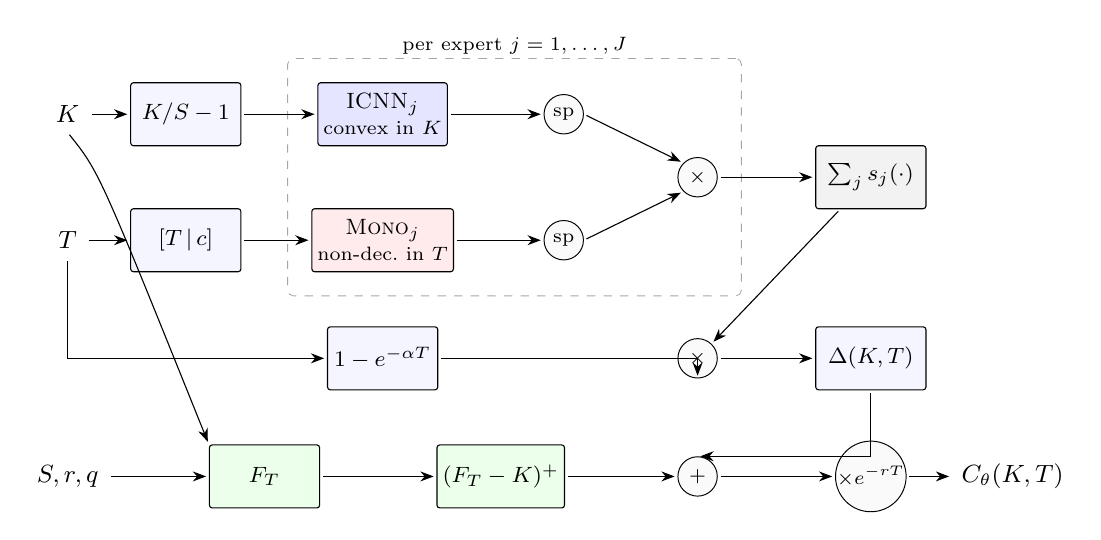
\begin{tikzpicture}[
  every node/.style={font=\small},
  block/.style    = {rectangle, draw=black, fill=blue!4, minimum width=14mm, minimum height=8mm, inner sep=2pt, align=center, line width=0.4pt, rounded corners=1pt, font=\footnotesize},
  cvxblock/.style = {block, fill=blue!10},
  monblock/.style = {block, fill=red!8},
  greenblock/.style = {block, fill=green!8},
  greyblock/.style = {block, fill=gray!10},
  oper/.style     = {circle, draw=black, fill=gray!4, inner sep=0pt, minimum size=5mm, line width=0.35pt, font=\scriptsize},
  io/.style       = {font=\small\bfseries, align=center},
  arrow/.style    = {-Stealth, line width=0.4pt, shorten >=1pt, shorten <=1pt},
  groupbox/.style = {draw=black!35, dashed, line width=0.3pt, inner sep=3mm, rounded corners=2pt}
]
%% TOP ROW: per-expert computation
\node[io]       (Kin)  at ( 0,    2.3) {$K$};
\node[block]    (Kn)   at ( 1.5,  2.3) {$K/S - 1$};
\node[cvxblock] (icnn) at ( 4.0,  2.3) {\icnn$_j$ \\ \scriptsize convex in $K$};
\node[oper]     (spK)  at ( 6.3,  2.3) {sp};
\node[oper]     (prodj)at ( 8.0,  1.5) {$\times$};
\node[greyblock](sum)  at (10.2,  1.5) {$\sum_j s_j (\cdot)$};

\node[io]       (Tin)  at ( 0,    0.7) {$T$};
\node[block]    (cat)  at ( 1.5,  0.7) {$[T \,|\, c]$};
\node[monblock] (mono) at ( 4.0,  0.7) {\mononet$_j$ \\ \scriptsize non-dec.\ in $T$};
\node[oper]     (spT)  at ( 6.3,  0.7) {sp};

%% BOTTOM ROW: assembly
\node[block]    (bnd)  at ( 4.0, -0.8) {$1 - e^{-\alpha T}$};
\node[oper]     (prod2)at ( 8.0, -0.8) {$\times$};
\node[block]    (delta)at (10.2, -0.8) {$\Delta(K, T)$};

\node[io]       (Pin)  at ( 0,   -2.3) {$S, r, q$};
\node[greenblock](FT)  at ( 2.5, -2.3) {$F_T$};
\node[greenblock](intr)at ( 5.5, -2.3) {$(F_T-K)^+$};
\node[oper]     (plus) at ( 8.0, -2.3) {$+$};
\node[oper]     (disc) at (10.2, -2.3) {$\times e^{-rT}$};
\node[io]       (out)  at (12.0, -2.3) {$C_\theta(K, T)$};

%% Arrows
\draw[arrow] (Kin) -- (Kn);
\draw[arrow] (Kn) -- (icnn);
\draw[arrow] (icnn) -- (spK);
\draw[arrow] (Tin) -- (cat);
\draw[arrow] (cat) -- (mono);
\draw[arrow] (mono) -- (spT);
\draw[arrow] (spK.east) -- (prodj.north west);
\draw[arrow] (spT.east) -- (prodj.south west);
\draw[arrow] (prodj) -- (sum);
\draw[arrow] (Tin.south) |- (bnd.west);
\draw[arrow] (bnd.east)  -| (prod2.south);
\draw[arrow] (sum) -- (prod2);
\draw[arrow] (prod2) -- (delta);
\draw[arrow] (Pin) -- (FT);
\draw[arrow] (Kin.south) .. controls +(0.4,-0.5) .. (FT.north west);
\draw[arrow] (FT) -- (intr);
\draw[arrow] (intr) -- (plus);
\draw[arrow] (delta.south) |- (plus.north);
\draw[arrow] (plus) -- (disc);
\draw[arrow] (disc) -- (out);

\begin{pgfonlayer}{background}
  \node[groupbox, fit=(icnn)(spK)(mono)(spT)(prodj),
        label={[font=\scriptsize, yshift=-2pt]above:per expert $j = 1, \dots, J$}] {};
\end{pgfonlayer}
\end{tikzpicture}
\caption{Computational graph of \arbnet{}. Convex-in-$K$ pathway (blue) and monotone-in-$T$ pathway (red) feed a per-expert product (top), summed across $J$ experts. The smooth boundary factor $1 - e^{-\alpha T}$ multiplies the sum to give $\Delta(K, T)$. The intrinsic baseline $(F_T - K)^+$ (bottom) is added and the result is discounted by $e^{-rT}$ to produce the call price. By \cref{thm:arbitrage-free}, conditions \ref{cond:butterfly}--\ref{cond:intrinsic-bound} hold for every parameter setting.}
\label{fig:arch}
\end{figure}

The architecture has a small number of explicit components. We list them and motivate each.

\subsection{Formal definitions of the building blocks}

\paragraph{Input-convex network ($\icnn$).}
Fix depth $L$ and widths $(w_0, \dots, w_L)$ with $w_0 = 1$, $w_L = 1$. The input-convex recurrence of \citet{amos2017input} reads
\begin{equation}
\label{eq:icnn-recurrence}
z_{\ell+1} = \sigma\!\bigl( W^{(z)}_\ell z_\ell + W^{(x)}_\ell x + W^{(c)}_\ell c + b_\ell \bigr),
\quad z_0 = 0,\, x = K/S,
\end{equation}
where $\sigma$ is a convex non-decreasing activation (we use softplus), $c$ is an optional auxiliary context (left at zero in the baseline configuration), and the weight constraint
\begin{equation}
\label{eq:icnn-constraint}
W^{(z)}_\ell \in \R_{\geq 0}^{w_{\ell+1} \times w_\ell}
\end{equation}
is enforced by reparameterisation $W^{(z)}_\ell = \softplus(\widetilde W^{(z)}_\ell)$ for unconstrained $\widetilde W^{(z)}_\ell$. The output is $\phi^{\mathrm{cvx}}(x; c) \eqdef z_L$. We use $L = 2$ and width $64$ throughout. The recurrence has the key structural property:

\begin{proposition}[\icnn{} convexity, {\cite{amos2017input}}]
\label{prop:icnn-convexity}
$x \mapsto \phi^{\mathrm{cvx}}(x; c)$ is convex on $\R$ for every $c$.
\end{proposition}
The proof is by induction on $\ell$: the affine layer $W^{(z)}_\ell z_\ell + W^{(x)}_\ell x + W^{(c)}_\ell c + b_\ell$ is convex in $x$ if $z_\ell$ is convex (by the non-negativity constraint on $W^{(z)}_\ell$ and the convexity-preserving cone closure of \cref{lem:cone-closure}); the activation $\sigma$ is convex non-decreasing, so by \cref{lem:cvx-comp} the composition is convex.

\paragraph{Monotone network ($\mononet$).}
Fix depth $L'$ and widths $(w'_0, \dots, w'_{L'})$ with $w'_0 = 1 + d_c$, $w'_{L'} = 1$. The monotone recurrence of \citet{daniels2010monotone,sill1998monotonic} reads
\begin{equation}
\label{eq:mono-recurrence}
h_{\ell+1} = \sigma\!\bigl( V^{(m)}_\ell h^{(m)}_\ell + V^{(c)}_\ell h^{(c)}_\ell + d_\ell \bigr),
\end{equation}
with $V^{(m)}_\ell \in \R_{\geq 0}^{w'_{\ell+1} \times w^{(m)}_\ell}$ (softplus-reparameterised) and $V^{(c)}_\ell$ unconstrained. The activation $\sigma$ is non-decreasing (softplus). The output is $\phi^{\mathrm{mon}}(T; c) \eqdef h_{L'}$. We use $L' = 2$ and width $32$ throughout. Recent extensions of monotone networks --- including unconstrained monotonic neural networks \cite{wehenkel2019unconstrained}, the Lipschitz monotonic networks of \citet{runje2023constrained}, and the polynomial-spline-based monotone approximators of \citet{guo2021neural} --- could be used as drop-in replacements; we use the classical Daniels--Velikova construction for simplicity.

\begin{proposition}[\mononet{} monotonicity, {\cite{daniels2010monotone}}]
\label{prop:mono-monotonicity}
$T \mapsto \phi^{\mathrm{mon}}(T; c)$ is non-decreasing on $\R_{\geq 0}$ for every $c$.
\end{proposition}

\paragraph{Scalar gates.}
The boundary growth rate $\alpha_\theta = \softplus(\widetilde\alpha) > 0$ is a learned positive scalar that controls the speed at which the time-value factor $1 - e^{-\alpha_\theta T}$ leaves zero. The per-expert positive scales $s_{j,\theta} = \softplus(\widetilde s_j) > 0$ control the relative weighting of each expert. Both are unconstrained-parameterised by softplus.

\subsection{Motivating the design choices}
\label{sec:design-choices}

Several design choices in \cref{eq:headline,eq:headline-delta} merit explicit justification.

\paragraph{Why decompose into intrinsic plus correction?}
The decomposition $C_\theta = e^{-rT}\bigl[(F_T - K)^+ + \Delta_\theta\bigr]$ is more than cosmetic. It separates the part of the call price that is universal across models (the forward intrinsic, which is the no-arbitrage lower bound \ref{cond:intrinsic-bound}) from the part that encodes the time value of optionality. The architecture only needs to learn the time-value correction, which is necessarily non-negative on a no-arbitrage surface. This is a much more constrained learning problem than learning $C$ directly, and a more numerically stable one: the dynamic range of the time value is smaller than the dynamic range of the call price (which spans intrinsic plus zero for deep OTM to large values for deep ITM).

\paragraph{Why a mixture of products?}
A single ICNN-MonoNet product would give a separable correction $\Delta_\theta(K, T) = f(K) g(T)$. Empirical surfaces are not separable: the smile gets flatter as $T$ grows (consistent with the Lee asymptotic) and the ATM term structure has shape. A finite mixture of products is the simplest extension that breaks separability while preserving the structural constraints. With $J$ experts, the architecture can represent any tensor-rank-$J$ separable approximation, and \cref{thm:universal-approximation} establishes density at $J \to \infty$.

\paragraph{Why the boundary factor $1 - e^{-\alpha T}$?}
The expiry boundary condition \ref{cond:boundary-expiry} requires that $C_\theta(K, 0) = (S - K)^+$, which in our decomposition is equivalent to $\Delta_\theta(K, 0) = 0$. The factor $1 - e^{-\alpha_\theta T}$ vanishes at $T = 0$ and is smoothly non-decreasing in $T$; multiplying every term of $\Delta_\theta$ by this factor enforces the boundary without imposing any other restriction. The exponential form is the natural choice: it has a single learnable parameter ($\alpha$) controlling the rate, and its derivative is $\alpha_\theta e^{-\alpha_\theta T} > 0$ everywhere, which keeps the monotonicity-preserving property of \cref{lem:mono-product} usable.

\paragraph{Why softplus rather than ReLU?}
Softplus, $\softplus(u) = \log(1 + e^u)$, is convex non-decreasing and strictly positive. The strict positivity matters: it ensures that gradients propagate through the per-expert product even when the ICNN output is small, which makes training more stable in the early phases. ReLU would zero out gradients on a measure-zero set in principle but a non-trivial fraction in practice with finite-precision arithmetic. The convexity and monotonicity of softplus are inherited from $\log(1 + e^u)$ in the obvious way.

\paragraph{Why the call-price domain rather than implied-vol?}
This is the most important design choice and we discuss it in \cref{sec:why-call-domain}.

\subsection{Forward pass and computational complexity}

\Cref{alg:forward} gives the forward pass in pseudocode.

\begin{algorithm}[t]
\caption{\arbnet{} forward pass}
\label{alg:forward}
\begin{algorithmic}[1]
\Require strike vector $K$, maturity vector $T$, spot $S$, rate $r$, dividend yield $q$, parameters $\theta$
\Ensure call prices $C$
\State $F \gets S \cdot \exp((r-q) T)$; \quad $I \gets \max(F - K, 0)$
\State $x \gets ((K/S) - 1)\cdot \kappa$; \quad $u \gets [T \,\|\, c]$; \quad $\Delta \gets 0$
\For{$j = 1, \dots, J$}
   \State $f_j \gets \softplus(\phi^{\mathrm{cvx}}_j(x))$ \Comment{convex in $K$, $\geq 0$}
   \State $g_j \gets \softplus(\phi^{\mathrm{mon}}_j(u))$ \Comment{non-decreasing in $T$, $\geq 0$}
   \State $s_j \gets \softplus(\widetilde s_j)$; \quad $\Delta \gets \Delta + s_j f_j g_j$
\EndFor
\State $\alpha \gets \softplus(\widetilde\alpha)$; \quad $\Delta \gets S\,(1-\exp(-\alpha T))\,\Delta$
\State $C \gets \exp(-rT)\cdot(I + \Delta)$ \Return $C$
\end{algorithmic}
\end{algorithm}

The total parameter count is $J \cdot (P_{\icnn} + P_{\mononet}) + J + 1$, where $P_{\icnn}$ and $P_{\mononet}$ are the per-network parameter counts. For our default configuration ($J = 6$, ICNN $[64, 64]$, MonoNet $[32, 32]$), this evaluates to approximately $33{,}000$ parameters in the context-free setting, rising to approximately $43{,}000$ when a per-day context vector feeds the ICNN and monotone modules, as in the real-data study of \cref{sec:exp-real}. The forward-pass cost for a batch of size $B$ is $\mathcal{O}(B \cdot J \cdot (\mathrm{width}_{\icnn}^2 L + \mathrm{width}_{\mononet}^2 L'))$, which is asymptotically identical to a soft-penalty MLP; the structural constraints add no computational overhead, because the softplus reparameterisation of the ICNN's $W^{(z)}_\ell$ matrices is a fixed per-layer cost that does not scale with the batch size.

\subsection{Why the call-price domain rather than the implied-vol domain}
\label{sec:why-call-domain}

A natural alternative to our construction would parameterise the implied total variance $w_\theta(k, T)$ directly using ICNN/MonoNet building blocks, with $k = \log(K/F_T)$. The conversion from implied variance to call price is via the \bs{} formula and is therefore one-to-one. However, the static-arbitrage conditions in the implied-vol domain are not preserved by simple compositions. The Durrleman positivity \cite{gatheral2014arbitrage,jacquier2014arbitrage} reads
\begin{equation}
\label{eq:durrleman}
g(k, T) \eqdef \left( 1 - \frac{k\,\partial_k w}{2w}\right)^2 - \frac{(\partial_k w)^2}{4}\!\left( \frac{1}{w} + \frac{1}{4}\right) + \frac{\partial^2_k w}{2} \geq 0,
\end{equation}
which is a non-linear functional of $w$ and its first two derivatives. Convexity of $w$ in $k$ implies the third term is non-negative, but does not imply the whole expression is non-negative; one can produce convex $w$ for which $g(k, T) < 0$ at some $k$. The implied-vol-domain construction therefore reduces to either (a) imposing the Durrleman condition as a soft penalty (recovering the soft-penalty paradigm) or (b) restricting to parameterisations like SVI where the Durrleman condition is implied by simpler parameter constraints, which limits expressivity.

In the call-price domain, by contrast, the no-arbitrage conditions \ref{cond:butterfly}--\ref{cond:intrinsic-bound} are first-order linear (convexity in $K$, monotonicity in $T$ of $e^{rT}C$). These properties are preserved by the elementary compositions used in \cref{eq:headline-delta} (non-negative weighted sums, products of non-negative monotone functions, composition with convex non-decreasing scalar functions). The call-price domain therefore admits a structural neural pricer with simple primitives; the implied-vol domain does not.

\subsection{Greeks via automatic differentiation}
\label{sec:greeks-overview}

Once the architecture is trained, all of the standard Greeks are computed by automatic differentiation \cite{baydin2018autodiff} of $C_\theta$ with respect to its inputs, using PyTorch's autograd \cite{paszke2019pytorch}. Specifically:
\begin{itemize}[leftmargin=1.5em]
\item Delta $\delta(K, T) = \partial_S C_\theta$ (single backward pass).
\item Gamma $\gamma(K, T) = \partial^2_K C_\theta = e^{-rT}\rho_T(K)$ (double backward pass). Structurally non-negative by \cref{thm:arbitrage-free}\,\ref{cond:butterfly}.
\item Theta $\Theta(K, T) = -\partial_T C_\theta$ (single backward pass).
\item Vega $\nu(K, T) = \partial_\sigma C_\theta\big|_{\sigma = \widehat\sigma(K, T)}$ (requires Newton inversion to obtain $\widehat\sigma$; see \cref{app:newton}).
\end{itemize}
The non-negativity of $\gamma$ is a guarantee \emph{absent} from soft-penalty pricers; it means that the delta is non-decreasing in strike (deeper out-of-the-money calls have smaller delta than at-the-money ones), which is a desirable monotonicity property for hedging stability. We discuss this further in \cref{sec:hedging-results}.

%==============================================================================
\section{Theoretical guarantees}
\label{sec:theoretical-guarantees}

\subsection{Auxiliary lemmas}

We collect three elementary lemmas of convex analysis \cite{boyd2004convex}; their roles in the main theorem are flagged.

\begin{lemma}[Convexity composition]
\label{lem:cvx-comp}
If $f : \R \to \R$ is convex and $h : \R \to \R$ is convex non-decreasing, then $h \circ f$ is convex.
\end{lemma}
\begin{proof}
For $\lambda \in [0, 1]$ and $x, y \in \R$,
\begin{align*}
h(f(\lambda x + (1-\lambda) y)) &\leq h(\lambda f(x) + (1-\lambda) f(y)) && \text{(convexity of $f$, monotonicity of $h$)} \\
&\leq \lambda h(f(x)) + (1-\lambda) h(f(y)) && \text{(convexity of $h$)}.
\end{align*}
\qed
\end{proof}

\begin{lemma}[Cone closure of convex functions]
\label{lem:cone-closure}
Convex functions on a convex domain are closed under non-negative linear combinations and scalar multiplication by non-negative scalars. Formally, if $f_1, \dots, f_N$ are convex and $\lambda_1, \dots, \lambda_N \geq 0$, then $\sum_i \lambda_i f_i$ is convex.
\end{lemma}

\begin{lemma}[Monotone product]
\label{lem:mono-product}
If $u, v$ are non-negative non-decreasing functions on $D \subseteq \R$, then $uv$ is non-decreasing on $D$. In particular, for any non-negative non-decreasing $u_1, \dots, u_N$, $\prod_i u_i$ is non-decreasing.
\end{lemma}
\begin{proof}
For $x \leq y$,
\[
u(y)v(y) - u(x)v(x) = u(y)\bigl(v(y) - v(x)\bigr) + v(x)\bigl(u(y) - u(x)\bigr) \geq 0,
\]
by non-negativity and monotonicity of $u$ and $v$. The general statement follows by induction.
\qed
\end{proof}

\subsection{Structural arbitrage-freeness}
\label{sec:no-arb-theorem-formal}

\begin{theorem}[Arbitrage-freeness of \arbnet{}]
\label{thm:arbitrage-free}
Let $C_\theta$ be defined by \cref{eq:headline,eq:headline-delta} with $\phi^{\mathrm{cvx}}_j$ satisfying \cref{eq:icnn-recurrence,eq:icnn-constraint}, $\phi^{\mathrm{mon}}_j$ satisfying \cref{eq:mono-recurrence}, and $\alpha_\theta, s_{j,\theta} > 0$. Assume $r \geq q \geq 0$. Then conditions \ref{cond:butterfly}--\ref{cond:intrinsic-bound} of \cref{def:no-arb} hold for every $\theta \in \Theta$.
\end{theorem}

\begin{proof}
We prove each condition in turn.

\paragraph{Condition \ref{cond:butterfly}: convexity in strike.}
We show that $K \mapsto C_\theta(K, T)$ is convex on $\R$ for every fixed $T \geq 0$.

The forward intrinsic $(F_T - K)^+ = \max(F_T - K, 0)$ is convex in $K$ as the pointwise maximum of two affine functions; multiplication by the positive constant $e^{-rT}$ preserves convexity (\cref{lem:cone-closure}).

For the correction $\Delta_\theta(K, T)$, we need to show that $K \mapsto \Delta_\theta(K, T)$ is convex for every fixed $T$. The strike enters only through the inner ICNN compositions $\phi^{\mathrm{cvx}}_j(K/S)$. By \cref{prop:icnn-convexity}, $u \mapsto \phi^{\mathrm{cvx}}_j(u)$ is convex on $\R$. The affine substitution $u = K/S$ preserves convexity, so $K \mapsto \phi^{\mathrm{cvx}}_j(K/S)$ is convex. Softplus is convex non-decreasing, so by \cref{lem:cvx-comp}, $K \mapsto \softplus(\phi^{\mathrm{cvx}}_j(K/S))$ is convex.

For each $j$, the time-dependent factor $\softplus(\phi^{\mathrm{mon}}_j(T))$ is a constant in $K$ that is non-negative. The per-expert scale $s_{j,\theta}$ is non-negative. By \cref{lem:cone-closure}, the per-expert contribution
\[
K \mapsto s_{j,\theta}\,\softplus(\phi^{\mathrm{cvx}}_j(K/S))\,\softplus(\phi^{\mathrm{mon}}_j(T))
\]
is a non-negative scalar multiple of a convex function in $K$, hence convex in $K$. The mixture sum over $j$ is a non-negative linear combination of convex functions, hence convex (\cref{lem:cone-closure}). Multiplying by the constants $S$ and $1 - e^{-\alpha_\theta T}$ (both non-negative) preserves convexity. Therefore $K \mapsto \Delta_\theta(K, T)$ is convex.

Finally, $K \mapsto C_\theta(K, T) = e^{-rT}[(F_T - K)^+ + \Delta_\theta(K, T)]$ is a non-negative linear combination of two convex functions in $K$, hence convex.

\paragraph{Condition \ref{cond:calendar}: carry-adjusted calendar monotonicity.}
We show that $T \mapsto e^{rT} C_\theta(K, T)$ is non-decreasing on $[0, T_{\max}]$ for every fixed $K \geq 0$. From \cref{eq:headline},
\[
e^{rT} C_\theta(K, T) = (F_T - K)^+ + \Delta_\theta(K, T).
\]

For the intrinsic, $T \mapsto F_T = Se^{(r-q)T}$ is non-decreasing under the assumption $r \geq q$; consequently $T \mapsto F_T - K$ is non-decreasing, and the positive-part operator $z \mapsto z^+$ is non-decreasing, so $T \mapsto (F_T - K)^+$ is non-decreasing.

For the correction, the strike-dependent factor $\softplus(\phi^{\mathrm{cvx}}_j(K/S))$ is a non-negative constant in $T$. By \cref{prop:mono-monotonicity}, $T \mapsto \phi^{\mathrm{mon}}_j(T)$ is non-decreasing, and softplus is non-decreasing, so $T \mapsto \softplus(\phi^{\mathrm{mon}}_j(T))$ is non-decreasing. The product
\[
T \mapsto \softplus(\phi^{\mathrm{cvx}}_j(K/S))\,\softplus(\phi^{\mathrm{mon}}_j(T))
\]
is the product of a non-negative constant in $T$ and a non-negative non-decreasing function of $T$, hence non-negative non-decreasing in $T$ (this is the degenerate case of \cref{lem:mono-product}). Multiplying by $s_{j,\theta} > 0$ and summing over $j$ preserves non-negative non-decreasingness. Multiplying by the non-negative non-decreasing boundary factor $1 - e^{-\alpha_\theta T}$ (whose derivative is $\alpha_\theta e^{-\alpha_\theta T} > 0$) preserves non-decreasingness by \cref{lem:mono-product}. Multiplying by the positive constant $S$ preserves it. Therefore $T \mapsto \Delta_\theta(K, T)$ is non-decreasing.

Summing the two non-decreasing functions yields a non-decreasing function.

\paragraph{Condition \ref{cond:boundary-expiry}: expiry boundary.}
At $T = 0$: $F_0 = Se^{(r-q)\cdot 0} = S$, so $(F_0 - K)^+ = (S - K)^+$. The boundary factor is $1 - e^{-\alpha_\theta \cdot 0} = 0$, so $\Delta_\theta(K, 0) = 0$. Hence $C_\theta(K, 0) = e^{0}[(S - K)^+ + 0] = (S - K)^+$.

\paragraph{Condition \ref{cond:intrinsic-bound}: forward intrinsic lower bound.}
Every factor in the expression for $\Delta_\theta$ is non-negative: $S > 0$; $1 - e^{-\alpha_\theta T} \geq 0$ for $T \geq 0$; the $s_{j,\theta}$ are positive; both softplus terms are positive. Therefore $\Delta_\theta(K, T) \geq 0$, and
\[
C_\theta(K, T) = e^{-rT}[(F_T - K)^+ + \Delta_\theta(K, T)] \geq e^{-rT}(F_T - K)^+,
\]
which is the desired bound.
\qed
\end{proof}

\begin{corollary}[Implied risk-neutral density]
\label{cor:rnd}
For every $T > 0$ and $\theta \in \Theta$, the implied risk-neutral density of $S_T$ under $\Qm$, defined by Breeden--Litzenberger as
\[
\rho^\theta_T(K) \eqdef e^{rT} \partial^2_K C_\theta(K, T),
\]
is a non-negative Borel measure on $\R_{\geq 0}$. It decomposes as
\[
\rho^\theta_T \;=\; \delta_{F_T} \;+\; e^{rT}\,\partial^2_K \Delta_\theta(\cdot, T),
\]
a Dirac atom at the forward $K = F_T$, inherited from the kink of the intrinsic $(F_T - K)^+$, plus an absolutely continuous part with non-negative Lebesgue density $e^{rT}\partial^2_K \Delta_\theta \geq 0$. Because the correction $\Delta_\theta$ is everywhere twice differentiable, it cannot cancel the intrinsic kink: the atom persists for \emph{every} $T > 0$. \arbnet{} therefore assigns strictly positive risk-neutral probability to the event $\{S_T = F_T\}$. This is a genuine and inspectable modelling artifact of the call-domain construction --- it appears as the density spike in \cref{fig:fitted-slice}(d) --- and we revisit it among the limitations of \cref{sec:limitations}.
\end{corollary}

\subsection{Universal approximation}
\label{sec:universal-approximation}

\begin{definition}[Convex-monotone class]
\label{def:cvx-mon-class}
Let $\mathcal{C}_{\mathrm{cvx},\nearrow}(\mathcal{B})$ be the set of continuous functions $g : \mathcal{B} = [K_0, K_1] \times [0, T_{\max}] \to \R_{\geq 0}$ that are strike-convex (\emph{i.e.}, $K \mapsto g(K, T)$ is convex for every $T$), time-non-decreasing (\emph{i.e.}, $T \mapsto g(K, T)$ is non-decreasing for every $K$), and satisfy $g(K, 0) = 0$ for every $K$.
\end{definition}

\begin{lemma}[Tensor-product density with explicit rate]
\label{lem:tensor-density}
Let $g \in \mathcal{C}_{\mathrm{cvx},\nearrow}(\mathcal{B})$ and $\eps_1 > 0$. Set $\delta = \omega_g^{-1}(\eps_1)$ (the largest $\delta$ such that $\omega_g(\delta) \leq \eps_1$, where $\omega_g$ is the bivariate modulus of continuity of $g$). Let $\{\kappa_\ell\}_{\ell=0}^{M_K}$ and $\{\tau_n\}_{n=0}^{M_T}$ be uniform partitions of $[K_0, K_1]$ and $[0, T_{\max}]$ with $M_K = \lceil (K_1 - K_0)/\delta\rceil$ and $M_T = \lceil T_{\max}/\delta\rceil$. Then there exist non-negative coefficients $\lambda_{\ell,n} \geq 0$ such that
\begin{equation}
g_M(K, T) \eqdef \sum_{\ell=0}^{M_K} \sum_{n=0}^{M_T} \lambda_{\ell,n}\,(K - \kappa_\ell)^+\,(T - \tau_n)^+
\end{equation}
satisfies $\|g - g_M\|_\infty \leq 3\eps_1$ on $\mathcal{B}$.
\end{lemma}
The proof, deferred to \cref{app:tensor-density-proof}, has three steps: piecewise-linear interpolation of $\tau \mapsto g(K, \tau)$ at the breakpoints $\{\tau_n\}$ produces non-negative slopes $a_n(K) \geq 0$; piecewise-linear convex interpolation of $K \mapsto a_n(K)$ produces non-negative slopes $\beta_{n,\ell} \geq 0$; combining gives the rank-one decomposition.

\begin{lemma}[\icnn{} density on convex non-negative functions]
\label{lem:icnn-approx}
For any continuous convex function $u : [a, b] \to \R_{\geq 0}$ and any $\eta > 0$, there exists an ICNN $\phi$ as in \cref{eq:icnn-recurrence,eq:icnn-constraint} with softplus activations such that $\|u - \softplus(\phi)\|_\infty < \eta$.
\end{lemma}
Sketch: this is a corollary of the input-convex universal approximation theorem of Amos--Xu \citeyearpar{amos2017input}, with subsequent refinements in \cite{chen2018optimal,bunne2022supervised}. ICNNs with softplus activations are $L^\infty$-dense in continuous convex functions on a compact interval; composing with $\softplus(\widehat\phi - \log 2)$ produces the non-negative output.

\begin{lemma}[\mononet{} density with boundary]
\label{lem:mononet-approx}
For any continuous non-decreasing function $v : [0, T'] \to \R_{\geq 0}$ with $v(0) = 0$ and any $\eta > 0$, there exist $\alpha > 0$ and a monotone network $\psi$ with $\bigl\|v(T) - (1 - e^{-\alpha T})\softplus(\psi(T))\bigr\|_\infty < \eta$ on $[0, T']$.
\end{lemma}
Sketch: Daniels and Velikova \citeyearpar{daniels2010monotone} establish $L^\infty$-density of monotone networks on continuous non-decreasing functions on a compact interval. The boundary factor $1 - e^{-\alpha T}$ with $\alpha$ large enough approximates the unit step at $T = 0$, removing the boundary singularity in $v$. Combining gives the result; full details in \cref{app:icnn-mono-proof}.

\begin{theorem}[Universal approximation with explicit rate]
\label{thm:universal-approximation}
Let $g \in \mathcal{C}_{\mathrm{cvx},\nearrow}(\mathcal{B})$ and $\eps > 0$. Then there exists an \arbnet{} correction $\widehat g$ of the form \cref{eq:headline-delta} with $\|g - \widehat g\|_\infty < \eps$. Moreover, the number of mixture components required is $J = \mathcal{O}(\omega_g^{-1}(\eps/3)^{-2})$.
\end{theorem}

\begin{proof}
Apply \cref{lem:tensor-density} with $\eps_1 = \eps/9$ to obtain $g_M$ with $\|g - g_M\|_\infty \leq \eps/3$ and $J = (M_K + 1)(M_T + 1) \leq C\omega_g^{-1}(\eps/9)^{-2}$. Each rank-one term $\lambda_{\ell,n}(K - \kappa_\ell)^+(T - \tau_n)^+$ has a strike factor $(K - \kappa_\ell)^+$ that is continuous convex non-negative on $[K_0, K_1]$, and a time factor $(T - \tau_n)^+$ that is continuous non-decreasing non-negative on $[0, T_{\max}]$ with value zero at $T = 0$.

Apply \cref{lem:icnn-approx} to approximate each $(K - \kappa_\ell)^+$ to within $\eta = \eps/(3J\overline{uv})$ in $L^\infty$, where $\overline{uv}$ is the maximum of $u_\ell v_n$ over the partition (a finite constant depending on $g$ and $\mathcal{B}$). Apply \cref{lem:mononet-approx} with a shared $\alpha$ to approximate each $(T - \tau_n)^+$ to within the same $\eta$. The product of two approximations is within $\eta \cdot \max + \max \cdot \eta = 2\eta \cdot \max$ of the true product, and summing $J$ such terms with non-negative coefficients $\lambda_{\ell,n}$ keeps the bound at $\|g_M - \widehat g\|_\infty \leq \eps/3$ by triangle inequality.

Combining via triangle inequality, $\|g - \widehat g\|_\infty \leq \|g - g_M\|_\infty + \|g_M - \widehat g\|_\infty \leq 2\eps/3 < \eps$.
\qed
\end{proof}

\subsection{Expressivity limit and the BS exclusion}
\label{sec:expressivity-limit}

\Cref{thm:universal-approximation} states that the architecture is universal on the class $\mathcal{C}_{\mathrm{cvx},\nearrow}$. It is, however, \emph{not universal} on the strictly larger class of all arbitrage-free call surfaces, because not every arbitrage-free call surface has a convex time-value in $K$. The most striking instance is the \bs{} family.

\begin{proposition}[\bs{} surfaces are not representable]
\label{prop:bs-excluded}
Let $C^{\mathrm{BS}}(K, T; \sigma)$ be the \bs{} call price with constant volatility $\sigma > 0$ and rates $r \geq q \geq 0$. Then $C^{\mathrm{BS}}(\cdot, \cdot; \sigma)$ does not lie in the image of the parameterisation \cref{eq:headline,eq:headline-delta} for any $\theta \in \Theta$.
\end{proposition}

\begin{proof}
The forward time value of \bs{} is
\[
\widetilde\Delta^{\mathrm{BS}}(K, T; \sigma) \eqdef e^{rT}C^{\mathrm{BS}}(K, T; \sigma) - (F_T - K)^+.
\]
This quantity is the difference between two quantities: (i) the carry-adjusted call price, which is smooth and strictly increasing in $T$, and (ii) the intrinsic, which has a non-differentiable kink at $K = F_T$. At $K = F_T$, the kink contribution makes $\widetilde\Delta^{\mathrm{BS}}$ attain its global maximum in $K$ (because the time value is maximised at-the-money under \bs{} for any $T > 0$ and $\sigma > 0$, a standard textbook result \cite{hull2018options}).

A function that attains a strict local maximum on an open set cannot be convex on that set. Therefore $K \mapsto \widetilde\Delta^{\mathrm{BS}}(K, T; \sigma)$ is non-convex on any open neighbourhood of $K = F_T$.

By \cref{thm:arbitrage-free}\,\ref{cond:butterfly}, an \arbnet{}-realised correction $\Delta_\theta(K, T)$ is convex in $K$ for every $\theta$. Two functions that differ in their convexity class cannot coincide on an open set. Therefore the parameterisation cannot represent \bs{}.
\qed
\end{proof}

Proposition~\ref{prop:bs-excluded} is the structural cost of the architectural compliance: by hard-coding convexity in $K$ into the architecture, we exclude any surface whose forward time-value is non-convex in $K$. This includes the entire \bs{} family, and more generally any surface where the time-value is bell-shaped (peaking at-the-money and decaying in both directions). Rough-Bergomi surfaces have less pronounced bell shapes than \bs{} at short maturities but still some; the empirical signature of this restriction appears in \cref{fig:fitted-slice}, where ArbNet's risk-neutral density is over-concentrated at the money.

It is worth noting that no \emph{soft-penalty} pricer has this exclusion: the soft-penalty MLP can represent any surface, just not without residual violations. The exclusion is therefore the explicit cost of the architectural-vs-penalty trade.

\subsection{The Lee wing slope}
\label{sec:lee-wing-slope}

A separate observation concerns the asymptotic shape of the smile. The Lee moment formula \cite{lee2004moment,lee2005implied}, recalled in \cref{sec:lee-wings}, requires the right-wing total variance to grow at most linearly in log-moneyness, with slope at most $2$. Our parameterisation does not enforce this bound structurally: in principle, the ICNN $\phi^{\mathrm{cvx}}_j$ can produce a quadratic or super-linear growth in $K/S$, which translates to a super-linear growth in $w(k, T)$ at large $|k|$. In practice, we observe that even untrained ICNNs (initialised with small weights) produce slopes well below 2, and trained ICNNs on data covering $\pm 30\%$ moneyness remain bounded. For training on data covering deeper wings ($\pm 50\%$ or more), one can mitigate by soft clamping of the last-layer ICNN weights, or by penalising the empirical wing slope with a weak regulariser. We do not pursue this in the present study because our training data is confined to the $\pm 30\%$ moneyness band where the issue does not arise.

%==============================================================================
\section{Training objective and algorithms}
\label{sec:training}

\subsection{Loss function}
\label{sec:loss}

Given a batch $\mathcal{D} = \{(K_i, T_i, C^{\mathrm{obs}}_i, c_i)\}_{i=1}^N$ of strike-maturity quotes (with optional context $c_i$), we define the total training loss as
\begin{equation}
\label{eq:total-loss}
\mathcal{L}_{\mathrm{total}}(\theta) = \mathcal{L}_{\mathrm{price}}(\theta) + \lambda_{\mathrm{IV}}\,\mathcal{L}_{\mathrm{IV}}(\theta) + \lambda_{\mathrm{hedge}}\,\mathcal{L}_{\mathrm{hedge}}(\theta),
\end{equation}
where the three terms are the vega-weighted price RMSE, the implied-volatility RMSE (optional), and the deep-hedging CVaR$_{0.95}$ (optional). Crucially, \emph{no soft no-arbitrage penalty is required}: the parameterisation is structurally compliant by \cref{thm:arbitrage-free}. The Ackerer-style baseline used for comparison adds a penalty term $\lambda_{\mathrm{arb}}\mathcal{L}_{\mathrm{arb}}$, while \arbnet{} sets $\lambda_{\mathrm{arb}} = 0$.

\subsection{Vega-weighted price loss}
\label{sec:vega-weighting}

The price loss is
\begin{equation}
\label{eq:price-loss}
\mathcal{L}_{\mathrm{price}}(\theta) = \frac{1}{N}\sum_{i=1}^N \frac{(C_\theta(K_i, T_i) - C^{\mathrm{obs}}_i)^2}{\max(\nu(K_i, T_i)^2, w_{\min}^2)},
\end{equation}
where $\nu(K_i, T_i)$ is the \bs{} vega evaluated at the observed implied volatility $\sigma^{\mathrm{obs}}_i$ and $w_{\min} > 0$ is a floor. The vega weighting reflects the standard market-practitioner observation that pricing errors in the wings (where $\nu$ is small) are much smaller than pricing errors near the money in absolute terms but comparable in volatility space; weighting by vega-squared converts the price RMSE into a quantity that is approximately proportional to the implied-volatility RMSE. The floor $w_{\min}$ prevents the loss from blowing up at deep-OTM quotes where vega is essentially zero; we use $w_{\min} = 10^{-3}$ throughout.

\subsection{Implied volatility loss (optional)}
\label{sec:iv-loss}

The implied-volatility loss is
\begin{equation}
\label{eq:iv-loss}
\mathcal{L}_{\mathrm{IV}}(\theta) = \frac{1}{N}\sum_{i=1}^N \bigl(\widehat\sigma_\theta(K_i, T_i) - \sigma^{\mathrm{obs}}_i\bigr)^2,
\end{equation}
where $\widehat\sigma_\theta$ is the Newton-inverted \bs{} implied volatility of the model price $C_\theta(K_i, T_i)$. The inversion is detailed in \cref{app:newton}. We disable the IV loss ($\lambda_{\mathrm{IV}} = 0$) in our experiments for two reasons: (i) the Newton inversion is unstable at deep wings, producing NaN gradients that propagate; and (ii) the vega-weighted price loss already approximates the IV-domain loss to first order. Empirically, enabling $\lambda_{\mathrm{IV}} > 0$ does not improve out-of-sample IV RMSE materially on rough-Bergomi surfaces and substantially increases training instability.

\subsection{Deep-hedging loss (optional)}
\label{sec:hedge-loss}

The deep-hedging loss \cite{buehler2019deep,chakrabarti2019deep,imaki2021no} simulates discrete delta hedging on Monte-Carlo paths under a market simulator (e.g., a calibrated rough-Bergomi process), and minimises a convex risk measure of the terminal hedged PnL:
\begin{equation}
\label{eq:hedge-loss}
\mathcal{L}_{\mathrm{hedge}}(\theta) = \mathrm{CVaR}_{0.95}\bigl[ -\Pi^{(p)}_\theta \bigr],
\end{equation}
where $\Pi^{(p)}_\theta$ is the PnL on path $p$ when hedging using $\partial_S C_\theta$ as the delta. The deep-hedging loss is more expensive to evaluate than the price loss because each minibatch requires a forward simulation of paths and accumulation of incremental hedges. We use $\lambda_{\mathrm{hedge}} = 0$ in our experiments and only compute the hedging diagnostic at evaluation time (\cref{alg:hedge}).

\subsection{Optimisation algorithm}
\label{sec:opt-algorithm}

We use Adam \cite{kingma2014adam,kingma2015adam} with learning rate $1\times10^{-2}$, batch size $64$, gradient clipping at $\ell_2$ norm $5.0$, and weight decay $10^{-6}$ for \arbnet{}; the same hyperparameters for the Ackerer baseline; and learning rate $2\times10^{-2}$ for the \bs{} baseline (a single-parameter model that converges faster). All weights are initialised with the Glorot/He scheme \cite{he2015delving} applied to the underlying unconstrained matrices $\widetilde W^{(z)}_\ell, V^{(m)}_\ell$, etc.; the softplus reparameterisation then projects into the constrained subspace.

\begin{algorithm}[t]
\caption{One epoch of \arbnet{} training}
\label{alg:train}
\begin{algorithmic}[1]
\Require dataset $\mathcal{D}$, batch size $B$, learning rate $\eta$, gradient clip $\gamma_{\mathrm{clip}}$, parameters $\theta$
\For{each mini-batch $\mathcal{B} \subset \mathcal{D}$}
  \State $C \gets \arbnet_\theta(\cdot)$ via \cref{alg:forward}
  \State $\mathcal{L} \gets \mathcal{L}_{\mathrm{price}} + \lambda_{\mathrm{IV}}\mathcal{L}_{\mathrm{IV}} + \lambda_{\mathrm{hedge}}\mathcal{L}_{\mathrm{hedge}}$
  \State $g \gets \nabla_\theta \mathcal{L}$, $g \gets g \cdot \min(1, \gamma_{\mathrm{clip}}/\|g\|_2)$
  \State $\theta \gets \mathrm{AdamStep}(\theta, g, \eta)$
\EndFor
\State \Return $\theta$
\end{algorithmic}
\end{algorithm}

\subsection{Static-arbitrage diagnostic}
\label{sec:diagnostic}

For evaluation, we report butterfly and calendar violation rates with a scale-aware tolerance $\tau_{\mathrm{tol}} = \max(10^{-7},\, 10^{-6}\cdot \bar C)$, where $\bar C$ is the mean call price across the diagnostic grid. Two precautions keep the diagnostic free of numerical artifacts. First, the diagnostic grid is evaluated in \emph{double} (float64) precision: in single precision, second differences of $5{,}000$-INR call prices can flag spurious sign changes of magnitude $10^{-5}$~INR on a structurally compliant surface, which would otherwise contaminate the violation counts. Second, the scale-aware tolerance discards any residual round-off below economic significance --- a violation of magnitude $10^{-8}$~INR on a $5{,}000$-INR call is an artifact of finite-precision arithmetic, not an arbitrage. The diagnostic is reported in \cref{alg:viol}.

\begin{algorithm}[t]
\caption{Scale-aware static-arbitrage diagnostic}
\label{alg:viol}
\begin{algorithmic}[1]
\Require pricer $\mathcal{M}$, strike grid $K[1{:}n_K]$, maturity grid $T[1{:}n_T]$, $(S, r, q)$, tolerance $\tau_{\mathrm{tol}}$
\Ensure $(n_{\mathrm{bf}}, n_{\mathrm{cal}})$, the violation counts
\State $C[i, j] \gets \mathcal{M}(K_j, T_i, S, r, q)$ for all $i, j$
\State $n_{\mathrm{bf}}, n_{\mathrm{cal}} \gets 0, 0$
\For{$i \in [1, n_T], j \in [2, n_K - 1]$}
  \State $\Delta^2 \gets (C_{i,j+1} - 2C_{i,j} + C_{i,j-1})/(\Delta K)^2$
  \If{$-\Delta^2 > \tau_{\mathrm{tol}}$} $n_{\mathrm{bf}} \gets n_{\mathrm{bf}} + 1$ \EndIf
\EndFor
\For{$i \in [1, n_T - 1], j \in [1, n_K]$}
  \If{$e^{rT_i} C_{i,j} - e^{rT_{i+1}}C_{i+1,j} > \tau_{\mathrm{tol}}$} $n_{\mathrm{cal}} \gets n_{\mathrm{cal}} + 1$ \EndIf
\EndFor
\State \Return $(n_{\mathrm{bf}}, n_{\mathrm{cal}})$
\end{algorithmic}
\end{algorithm}

\subsection{Delta-hedging diagnostic}
\label{sec:hedge-diagnostic}

The hedging diagnostic, \cref{alg:hedge}, simulates discrete delta-hedging on rough-Bergomi paths and reports the standard deviation and CVaR$_{0.95}$ of the terminal hedged PnL. The standard deviation is a measure of hedging precision; the CVaR$_{0.95}$ is a tail measure capturing the worst-case PnL over the worst 5\% of paths \cite{glasserman2003monte,glasserman2010sensitivity}.

\begin{algorithm}[t]
\caption{Delta-hedge PnL simulation}
\label{alg:hedge}
\begin{algorithmic}[1]
\Require pricer $\mathcal{M}$, paths $\{S^{(p)}_t\}$, strike $K$, maturity $T_{\mathrm{hedge}}$, implied vol $\widehat\sigma$, step $dt$, cost $\tau$
\For{$p = 1, \dots, P$}
  \State $V_0 \gets \mathcal{M}(K, T_{\mathrm{hedge}}, S^{(p)}_0)$; $\delta_0 \gets \partial_S \mathcal{M}(\cdot)$
  \State $\mathrm{cash}_0 \gets V_0 - \delta_0 S^{(p)}_0$
  \For{$t = 1, \dots, n_t$}
    \State $\delta_t \gets \partial_S\mathcal{M}(K, T_{\mathrm{hedge}} - t\,dt, S^{(p)}_t)$
    \State $\mathrm{cash}_t \gets e^{r\,dt}\mathrm{cash}_{t-1} - (\delta_t - \delta_{t-1}) S^{(p)}_t - \tau|\delta_t - \delta_{t-1}|S^{(p)}_t$
  \EndFor
  \State $\Pi^{(p)} \gets \mathrm{cash}_{n_t} + \delta_{n_t} S^{(p)}_{n_t} - (S^{(p)}_{n_t} - K)^+$
\EndFor
\State \Return $\{\Pi^{(p)}\}$
\end{algorithmic}
\end{algorithm}

%==============================================================================
\section{Experimental setup}
\label{sec:experimental-setup}

\subsection{Synthetic surface generation}
\label{sec:data-gen}

We generate synthetic call surfaces from a rough-Bergomi process \cite{bayer2016pricing,bayer2023primer}. The rough-Bergomi model is a path-dependent stochastic volatility model in which the log-volatility is driven by a fractional Brownian motion of Hurst parameter $H < 1/2$; the corresponding instantaneous variance process is the exponential of a centred Gaussian process with covariance reflecting the roughness of the volatility paths. The model is calibrated to capture three stylised facts of equity-index volatility surfaces: (i) ATM volatility skew that decays with maturity at a rate $T^{H - 1/2}$ for $H < 1/2$, which empirically matches the observed short-end behaviour; (ii) a non-zero wing slope at short maturities, captured by the $\rho$ parameter; (iii) an ATM term-structure that decays towards a long-run level, captured by the initial variance curve $\xi_0(\cdot)$.

For our experiments we use a constant initial variance $\xi_0(t) = \xi_0$. The rough-Bergomi parameters are drawn from
\begin{align*}
H &\in [0.07, 0.20] \quad &&\text{(roughness)} \\
\eta &\in [1.0, 3.0] \quad &&\text{(vol-of-vol)} \\
\rho &\in [-0.9, -0.3] \quad &&\text{(spot-vol correlation)} \\
\xi_0 &\in [0.02, 0.10] \quad &&\text{(initial variance)}.
\end{align*}
Each draw defines one surface. We sample 10 distinct surfaces from this grid. For each surface, we use the hybrid scheme of Bennedsen, Lunde, and Pakkanen \citeyearpar{bennedsen2017hybrid} to simulate $4{,}000$ Monte-Carlo paths of the rough-Bergomi process. We then price European calls on a grid of 20 strikes spanning $\pm 30\%$ moneyness in 5 maturities $(7, 14, 30, 60, 90)$ days, for a total of $100$ quotes per surface. The spot is $S = 20{,}000$ (matching Nifty-50 scale in INR), the risk-free rate is $r = 6.5\%$ (matching the Indian repo rate of mid-2024), and the dividend yield is $q = 1.2\%$ (matching the Nifty-50 trailing yield).

For each surface, we run three independent training seeds. The total number of (surface, seed) trials is therefore $30$.

\subsection{Real NSE Nifty~50 option data}
\label{sec:exp-real}

The real-data study runs a day-by-day walk-forward over the National Stock Exchange of India (NSE) Nifty~50 index-option market.

\paragraph{Primary data.}
The training data is the NSE Futures \& Options daily \emph{bhavcopy}: one file per trading day giving the settlement price, open interest, and volume of every listed contract. We retain the Nifty~50 index calls and take the official settlement price as the quote. The sample spans $1{,}359$ trading days, 1~January 2019 to 5~July 2024, and therefore covers the COVID-19 crash of early 2020 and the post-2022 monetary-tightening cycle. The underlying spot $S$ is the official Nifty~50 daily close; the risk-free rate $r$ is the cut-off yield of the most recent 91-day Government of India Treasury-bill auction on or before each date; the dividend yield $q$ is the NSE Nifty~50 factsheet yield. Every series is committed to the paper's repository, so the study runs with no network access.

\paragraph{Quality filtering.}
Deep-out-of-the-money weekly options on NSE frequently carry stale settlement prices after volatility spikes. Before fitting, each daily cross-section is passed through a fixed quality filter that drops contracts with a settlement price below $0.05$~INR, with $|\log(K/F)| > 0.5$, or that violate the elementary no-arbitrage price bounds. Per-contract implied volatilities are then obtained from the surviving quotes by the vectorised Newton inversion of \cref{app:newton}. No trading day in the sample is discarded by the pipeline: all $1{,}359$ days are fitted and evaluated.

\paragraph{Context features.}
Because \arbnet{} is arbitrage-free for \emph{every} context vector (\cref{thm:arbitrage-free}), it is safe to condition the ICNN and monotone modules on auxiliary market state. We assemble a ten-dimensional per-day context vector: India VIX, an at-the-money Bank Nifty implied volatility computed on the fly from the same bhavcopy, one-week realised volatility of the Nifty~50, the USD/INR rate, foreign- and domestic-institutional net cash-market flows, headline CPI and WPI inflation, IIP growth, and the number of calendar days to the next scheduled macroeconomic event. The monthly macro series are lagged to their real publication dates to avoid look-ahead bias. The vector is $z$-scored and supplied to \arbnet{} only; the soft-penalty and \bs{} baselines are context-free.

\paragraph{Walk-forward protocol.}
On each of the $1{,}359$ days the three models are fitted independently on that day's filtered cross-section and evaluated the same day. Static-arbitrage compliance is measured by differencing model prices on a $41$-strike by multi-maturity grid; following the diagnostic of \cref{sec:diagnostic}, the grid is evaluated in \emph{float64} so that the violation counts are not contaminated by float-32 round-off. We report the butterfly and calendar rates as \emph{guaranteed} quantities for \arbnet{} --- they are zero by \cref{thm:arbitrage-free} for every weight vector and every context --- and the Roger Lee wing/tail bound as a \emph{monitored} diagnostic, since it is not enforced by the architecture (\cref{sec:lee-wing-slope}). Per-day delta-hedging statistics are computed on a fresh rough-Bergomi resimulation.

\subsection{Model architectures}
\label{sec:model-arch}

We train three models per (surface, seed) trial.

\paragraph{\arbnet{}.}
The construction of \cref{eq:headline,eq:headline-delta} with $J = 6$ mixture experts, each comprising an ICNN of depth $L = 2$ and width $64$ and a monotone network of depth $L' = 2$ and width $32$; activations are softplus throughout and no arbitrage penalty is applied ($\lambda_{\mathrm{arb}} = 0$). The model has approximately $33{,}000$ parameters, rising to about $43{,}000$ in the context-conditioned configuration used for the real-data study.

\paragraph{\ackerer{} (soft-penalty baseline).}
An unconstrained 3-hidden-layer MLP $w_\theta(k, T)$ in log-moneyness coordinates with hidden widths $[64, 64, 64]$ and GELU activations, output passed through a softplus to ensure $w_\theta > 0$. Implied variance is converted to a call price via the \bs{} formula. The soft penalty $\lambda_{\mathrm{arb}}\mathcal{L}_{\mathrm{arb}}$ with $\lambda_{\mathrm{arb}} = 1.0$ is evaluated on a $21$-strike by multi-maturity training grid spanning the moneyness and maturity range of the data. The baseline has approximately $8{,}600$ parameters. We do not match parameter counts across architectures: the two models live in different domains (implied variance versus call price), and the comparison is designed to hold the optimiser, schedule, and training data fixed rather than the capacity. \arbnet{} in fact carries the larger parameter budget, so any weaker price fit it exhibits is attributable to the convexity constraint and not to limited capacity.

\paragraph{\bs{}.}
A single-parameter \bs{} pricer with the volatility $\sigma$ as the sole learnable parameter, optimised by the same Adam routine as the others. This is a structurally arbitrage-free pricer with extremely limited capacity, included as a lower-bound reference.

\subsection{Training hyperparameters}
\label{sec:hyperparams}

All three models are trained on the same data per (surface, seed) trial. We use $150$ epochs for \arbnet{} and the Ackerer baseline; $80$ epochs for \bs{} (which converges faster). The batch size is $64$, gradient clipping is at $\ell_2$ norm $5.0$, and weight decay is $10^{-6}$. The learning rate is $1\times10^{-2}$ for \arbnet{} and Ackerer, and $2\times10^{-2}$ for \bs{}. The loss-weighting hyperparameters are $\lambda_{\mathrm{price}} = 1$, $\lambda_{\mathrm{IV}} = 0$, $\lambda_{\mathrm{hedge}} = 0$ for all three; $\lambda_{\mathrm{arb}} = 1$ for Ackerer, $0$ for the others. The full hyperparameter table is in \cref{app:hyperparams}.

\subsection{Evaluation metrics}
\label{sec:metrics}

For each (surface, seed) trial we report:

\begin{itemize}[leftmargin=1.5em]
\item \emph{Price RMSE} (INR): root-mean-square pricing error on the training grid. Lower is better. Reported in Nifty-50-scale INR.
\item \emph{Implied vol RMSE}: root-mean-square error in implied volatility, computed by Newton-inverting both the model price and the observed price.
\item \emph{Butterfly violation rate}: fraction of $(T, K)$ grid points failing condition \ref{cond:butterfly} at the scale-aware tolerance $\tau_{\mathrm{tol}}$. Reported on a $41$-strike evaluation grid (five maturities for the synthetic surfaces, the day's listed maturities for the real data), differenced in float64.
\item \emph{Calendar violation rate}: fraction failing condition \ref{cond:calendar}.
\item \emph{Hedge PnL std}: standard deviation of the terminal delta-hedged PnL over $500$ rough-Bergomi paths.
\item \emph{Hedge CVaR$_{0.95}$}: expected loss conditional on being in the worst 5\% tail.
\end{itemize}

\subsection{Hardware and reproducibility}
\label{sec:hardware}

All experiments run on a single CPU; no GPU is required. The $30$-trial synthetic study completes in under two minutes; the full $1{,}359$-day real-data walk-forward, which fits and evaluates $3 \times 1{,}359$ models, completes in roughly eight CPU-hours. Every random seed is pinned --- the rough-Bergomi simulator, the data-loader shuffle, and the PyTorch and NumPy generators --- and the exact reproduction commands are given in \cref{sec:reproducibility}.

%==============================================================================
\section{Results}
\label{sec:results}

\subsection{The real-data walk-forward}
\label{sec:real-result}

The headline evidence is the $1{,}359$-day NSE Nifty~50 walk-forward; \cref{tab:real} collects it and \cref{fig:real-study} displays it.

\paragraph{Compliance.}
\arbnet{} records a butterfly violation rate and a calendar violation rate of \emph{exactly} zero on every one of the $1{,}359$ trading days --- zero days with any violation. This is not a fitted outcome but a direct empirical manifestation of \cref{thm:arbitrage-free}: the architecture is butterfly- and calendar-compliant for every weight vector and every context, so no training trajectory --- and no market regime in the 2019--2024 sample, including the COVID-19 crash --- can produce a violation. The soft-penalty Ackerer baseline, by contrast, violates static arbitrage on $961$ of the $1{,}359$ days, $70.7\%$ of the sample. Its mean daily butterfly rate is $3.73\%$ of grid points, reaching $31.6\%$ on the worst day; its mean daily calendar rate is $1.14\%$, reaching $15.5\%$. The penalty weight ($\lambda_{\mathrm{arb}} = 1$) and the training budget are exactly those of the synthetic study; the soft penalty simply cannot hold the constraint on real, noisy cross-sections the way it nearly does on smooth synthetic surfaces (\cref{sec:synth-result}). The \bs{} pricer is structurally compliant and records zero violations, as it must.

\paragraph{Fit.}
The guarantee is not free. \arbnet{}'s mean daily price RMSE is $95.16$~INR ($95\%$ confidence interval $[93.7, 96.6]$), against $36.17$~INR for the soft-penalty baseline and $39.72$~INR for \bs{}; the confidence intervals are tight and nowhere near overlapping. On the real data, then, \arbnet{} fits prices roughly $2.6$ times less accurately than the soft-penalty baseline, a gap of $58.98$~INR per call that is far larger, in relative terms, than the synthetic study alone would suggest. We take this seriously rather than minimise it: the fit cost is the subject of \cref{sec:pareto,sec:fitted-slice-results}, and its architectural cause --- the convexity restriction of \cref{prop:bs-excluded} --- is structural, not a training artifact.

\paragraph{The soft-penalty baseline is the harder comparison.}
It is worth stating plainly that the soft-penalty baseline is the strong competitor on fit and the weak one on compliance, while \bs{}, a one-parameter model, fits the real surface almost as well as the far larger soft-penalty network ($39.7$ against $36.2$~INR) --- a reminder that, on a liquid index with a single dominant at-the-money level, mean-squared price error is an easy target. The genuine contest in this paper is therefore \arbnet{} against the soft-penalty baseline: a hard compliance guarantee at a real fit cost, versus a better fit punctuated by violations on seven trading days in ten.

\begin{table}[t]
\centering
\caption{Real-data walk-forward over $1{,}359$ NSE Nifty~50 option-market days (1~January 2019 to 5~July 2024). Price and implied-volatility RMSE are means across days, with bootstrap $95\%$ confidence intervals; violation rates are means across days of the per-day fraction of $(T,K)$ grid points failing each condition; ``days with a violation'' counts days carrying at least one butterfly or calendar violation. The Lee-tail rate is monitored, not architecturally enforced. Hedging statistics are means of the per-day delta-hedge diagnostic.}
\label{tab:real}
\begin{tabular}{lccc}
\toprule
 & \arbnet{} & \ackerer{} & \bs{} \\
\midrule
Price RMSE (INR)             & $95.16$            & $36.17$            & $39.72$ \\
\quad bootstrap $95\%$ CI    & $[93.7,\,96.6]$    & $[35.1,\,37.3]$    & $[38.8,\,40.6]$ \\
IV RMSE                      & $0.104$            & $0.078$            & $0.069$ \\
Butterfly violation rate     & $\mathbf{0.000\%}$ & $3.730\%$          & $0.000\%$ \\
Calendar violation rate      & $\mathbf{0.000\%}$ & $1.141\%$          & $0.000\%$ \\
Days with a violation        & $\mathbf{0}/1359$  & $961/1359$         & $0/1359$ \\
Monitored Lee-tail rate      & $0.140\%$          & $0.517\%$          & $0.000\%$ \\
Hedge PnL std (INR)          & $175.9$            & $125.1$            & $124.2$ \\
Hedge $\mathrm{CVaR}_{95}$ (INR) & $728.2$        & $338.0$            & $322.8$ \\
\bottomrule
\end{tabular}
\end{table}

\begin{figure}[t]
\centering
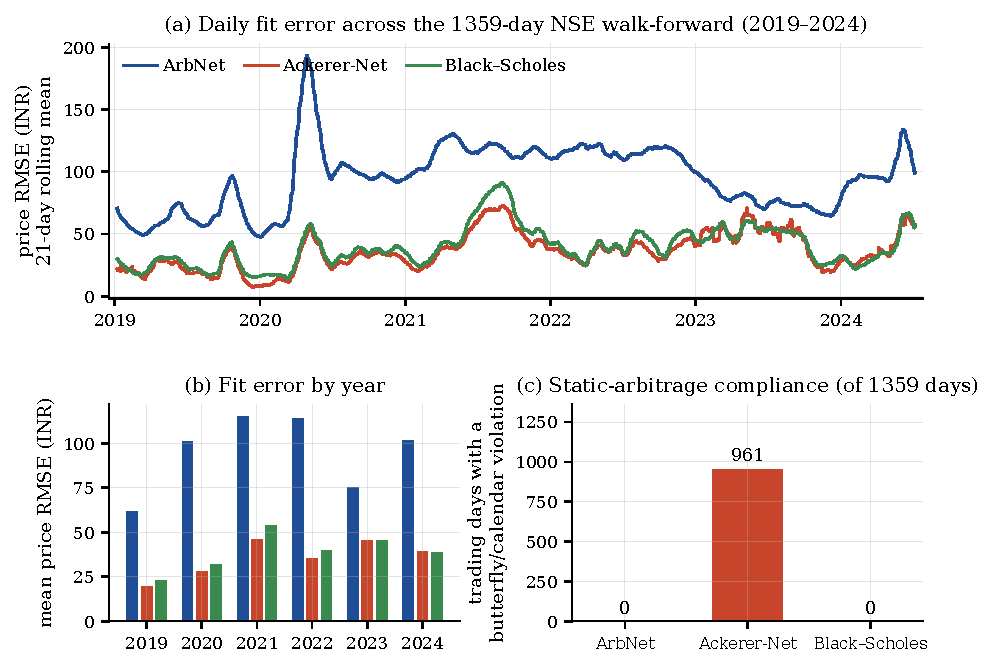
\includegraphics[width=\textwidth]{figures/fig2_real_study.pdf}
\caption{The real-data walk-forward over $1{,}359$ NSE Nifty~50 option-market days. \textbf{(a)}~Twenty-one-day rolling mean of the daily price RMSE, 2019--2024. \textbf{(b)}~Mean price RMSE by calendar year. \textbf{(c)}~Number of trading days, out of $1{,}359$, on which each model commits at least one butterfly or calendar violation: zero for \arbnet{} by \cref{thm:arbitrage-free}, $961$ for the soft-penalty baseline, zero for the structurally compliant \bs{} pricer.}
\label{fig:real-study}
\end{figure}

\subsection{The synthetic controlled study}
\label{sec:synth-result}

\Cref{tab:main} reports the $30$-trial synthetic study, which serves as a controlled complement: the rough-Bergomi data-generating process is arbitrage-free and smooth by construction, so it isolates the architectures from the noise of real quotes.

Three observations follow. First, \arbnet{} again records identically zero butterfly and calendar violations on every trial. Second, the soft-penalty baseline is \emph{far} better behaved here than on real data: its mean butterfly rate is only $0.154\%$ --- a handful of grid points on a few of the harder surfaces --- and its calendar rate is zero. The contrast with the $961$ violation days of the real study is the central methodological point: a synthetic benchmark, however carefully constructed, materially understates the failure mode of soft-penalty enforcement, and only real, noisy cross-sections expose it. Third, \arbnet{}'s mean price RMSE ($134.27$~INR) again exceeds the soft-penalty baseline's ($78.05$~INR), with a paired $t$-statistic of $3.71$ over the $30$ trials. The \bs{} pricer attains the lowest synthetic RMSE ($37.40$~INR): on benign rough-Bergomi smiles within our parameter ranges a single at-the-money volatility captures the bulk of the price variation, and the residual smile mismatch is small in absolute price terms even though it is large in implied-volatility terms. This is not a defence of \bs{} as a production pricer --- on the real Nifty~50 surface its skew mismatch is far more costly --- but a caution that synthetic RMSE comparisons flatter low-capacity models.

\begin{table}[t]
\centering
\caption{Synthetic controlled study: $30$ (surface, seed) trials over $10$ rough-Bergomi surfaces. Mean $\pm$ standard deviation across trials. Violation rates are fractions of $(T,K)$ grid points failing each condition at the scale-aware tolerance, on the float64 diagnostic grid. Hedging statistics are from $500$ rough-Bergomi paths per trial.}
\label{tab:main}
\begin{tabular}{lccc}
\toprule
 & \arbnet{} & \ackerer{} & \bs{} \\
\midrule
Price RMSE (INR)             & $134.27 \pm 39.56$ & $78.05 \pm 62.53$  & $37.40 \pm 12.70$ \\
IV RMSE                      & $0.127 \pm 0.033$  & $0.086 \pm 0.143$  & $0.066 \pm 0.016$ \\
Butterfly violation rate     & $\mathbf{0.000\%}$ & $0.154\%$          & $0.000\%$ \\
Calendar violation rate      & $\mathbf{0.000\%}$ & $0.000\%$          & $0.000\%$ \\
Hedge PnL std (INR)          & $272.9$            & $255.5$            & $161.8$ \\
Hedge $\mathrm{CVaR}_{95}$ (INR) & $1128.3$       & $834.3$            & $433.6$ \\
\bottomrule
\end{tabular}
\end{table}

\subsection{The fit--compliance frontier}
\label{sec:pareto}

\Cref{fig:pareto} places the two studies side by side in (violation rate, RMSE) coordinates. In both panels \arbnet{} sits exactly on the structural-zero edge --- the vertical axis at zero violation rate --- and no other model reaches it. The soft-penalty baseline sits at a strictly positive violation rate in both panels: marginally so on the synthetic surfaces, emphatically so on the real data. The frontier is the visual statement of the paper: moving compliance from a tolerance-bound regulariser to an architectural invariant has a price, measured on the vertical axis, and that price is paid in full and is reproducible.

\begin{figure}[t]
\centering
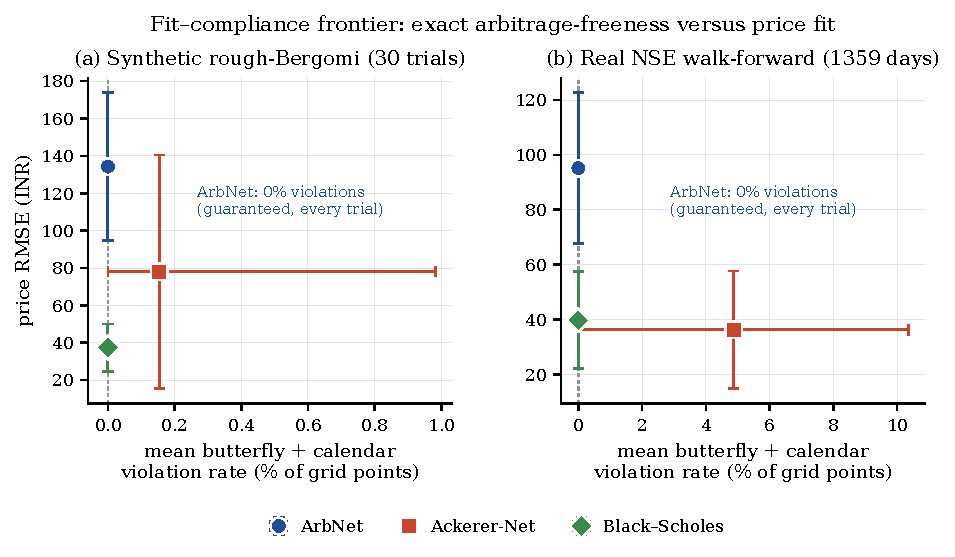
\includegraphics[width=\textwidth]{figures/fig1_pareto.pdf}
\caption{The fit--compliance frontier. Each panel plots the mean static-arbitrage violation rate (horizontal) against the mean price RMSE (vertical); bars are one standard deviation. \textbf{(a)}~The $30$-trial synthetic study. \textbf{(b)}~The $1{,}359$-day real NSE walk-forward. \arbnet{} sits exactly on the zero-violation edge in both panels --- a consequence of \cref{thm:arbitrage-free}, not of training --- while the soft-penalty baseline sits at a strictly positive violation rate, marginal on synthetic surfaces and pronounced on real data.}
\label{fig:pareto}
\end{figure}

No Pareto-improving point exists for \arbnet{}: at zero violation rate it is, by construction, the only model present. Whether its structural-zero edge is preferred over the soft-penalty baseline's operating point --- a violation on $70.7\%$ of days at a $36$-INR RMSE --- depends entirely on the loss function of the downstream consumer, a decision we formalise in \cref{sec:when-to-choose}.

\subsection{Where the fit gap comes from: a representative real fit}
\label{sec:fitted-slice-results}

\Cref{fig:fitted-slice} dissects a single real NSE snapshot --- 1~June 2023, spot $\approx 18{,}488$, the $\approx 28$-day maturity --- to show \emph{where} \arbnet{} loses the fit.

\begin{figure}[t]
\centering
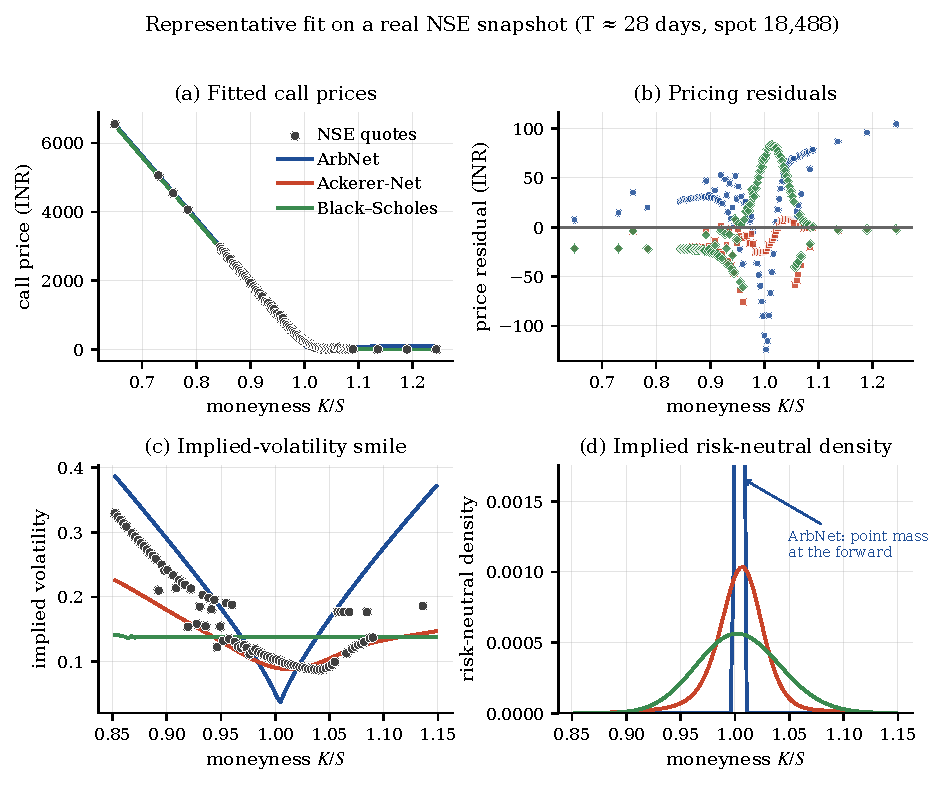
\includegraphics[width=\textwidth]{figures/fig3_fitted_slice.pdf}
\caption{A representative fit on one real NSE snapshot (1~June 2023, spot $\approx 18{,}488$, maturity $\approx 28$ days). \textbf{(a)}~Fitted call prices against the NSE quotes. \textbf{(b)}~Pricing residuals, model minus market. \textbf{(c)}~Implied-volatility smile. \textbf{(d)}~Implied risk-neutral density by centred finite differences; \arbnet{}'s curve is dominated by the Dirac atom at the forward of \cref{cor:rnd} (the off-scale spike), the vertical axis being clipped to keep the absolutely continuous parts of all three densities legible.}
\label{fig:fitted-slice}
\end{figure}

Panel~(a) shows that all three call-price curves track the quoted prices closely at the scale of the price itself; the differences live in the residuals of panel~(b), where \arbnet{} carries a systematic at-the-money error of order $100$~INR --- undershooting at the money, overshooting in the wings --- while the soft-penalty baseline and \bs{} stay closer to zero. Panel~(c) converts this to implied volatility: the quoted smile has a pronounced left skew, which the soft-penalty baseline tracks, whereas \arbnet{}'s smile is a sharp, near-symmetric V, dipping below the quotes at the money and rising steeply in both wings. This is the convexity restriction of \cref{prop:bs-excluded} made visible --- the architecture must fit the whole cross-section with a time value that is convex in strike, and a convex time value cannot reproduce a bell-shaped, skewed smile. Panel~(d) shows the implied risk-neutral density: the soft-penalty and \bs{} densities are smooth and bell-shaped, while \arbnet{}'s is dominated by the Dirac atom at the forward predicted by \cref{cor:rnd} --- the off-scale spike --- with little absolutely continuous mass elsewhere. The atom is the sharpest single illustration of the architectural cost: \arbnet{} buys a hard no-arbitrage guarantee but, on a skewed real surface, pays for it with a degenerate implied density.

\subsection{Hedging performance}
\label{sec:hedging-results}

\Cref{tab:real} also reports the delta-hedging diagnostic, and \cref{fig:hedge-pnl} shows a representative PnL distribution. Across the real walk-forward, \arbnet{}'s mean hedge-PnL standard deviation ($175.9$~INR) and $\mathrm{CVaR}_{95}$ ($728.2$~INR) are both materially worse than the soft-penalty baseline's ($125.1$ and $338.0$~INR) and \bs{}'s ($124.2$ and $322.8$~INR).

\begin{figure}[t]
\centering
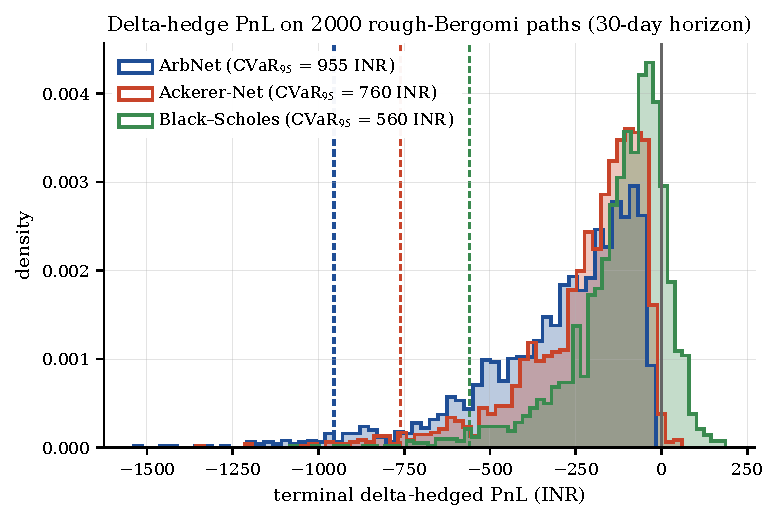
\includegraphics[width=0.78\textwidth]{figures/fig4_hedge_pnl.pdf}
\caption{Terminal delta-hedged PnL on $2{,}000$ rough-Bergomi paths over a $30$-day horizon, each model hedging at its own at-the-money implied volatility. Dashed lines mark $-\mathrm{CVaR}_{95}$ per model. \arbnet{}'s left tail is the heaviest: an implied density over-concentrated at the forward inflates its at-the-money gamma, so its delta over-reacts to small spot moves.}
\label{fig:hedge-pnl}
\end{figure}

The heavier \arbnet{} tail has the same root cause as the V-shaped smile of \cref{fig:fitted-slice}: an implied density over-concentrated at the forward inflates the at-the-money gamma, so the delta extracted from \arbnet{} over-reacts to small spot moves and accumulates tracking error. The hedging cost is therefore not separate from the fit cost --- it is the same architectural feature seen through a different diagnostic.

\subsection{Training behaviour}
\label{sec:training-behaviour}

\Cref{fig:convergence} shows the per-epoch training loss of the three models on the representative real snapshot. \arbnet{} starts from a large loss --- an untrained ICNN/monotone mixture produces wild prices --- but converges within roughly $20$ epochs and is flat thereafter; the soft-penalty baseline and \bs{} converge comparably. Panel~(b), the loss normalised by its epoch-one value, shows that \arbnet{} traverses a far larger dynamic range yet reaches a stable optimum on the same timescale as the baselines. We observe no instabilities --- no NaN gradients, no divergent losses --- at the stated hyperparameters. We did initially observe instabilities with the implied-volatility loss enabled ($\lambda_{\mathrm{IV}} > 0$), because the Newton inversion of model prices at deep wings produces NaN gradients that propagate through automatic differentiation; setting $\lambda_{\mathrm{IV}} = 0$, as we do throughout, removes them, and the vega-weighted price loss already approximates the implied-volatility objective to first order.

\begin{figure}[t]
\centering
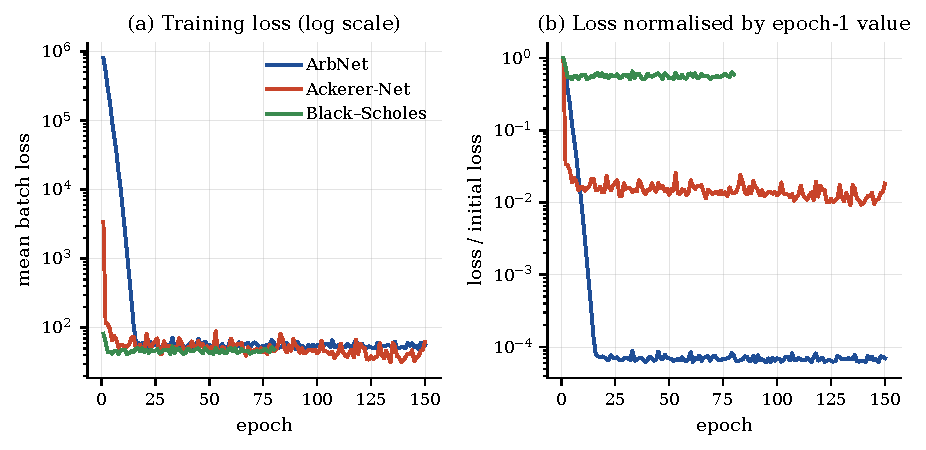
\includegraphics[width=\textwidth]{figures/fig5_convergence.pdf}
\caption{Training convergence on the representative real NSE snapshot. \textbf{(a)}~Mean batch loss per epoch, logarithmic scale. \textbf{(b)}~Loss normalised by its epoch-one value. \arbnet{} traverses a larger dynamic range but reaches a stable optimum on the same timescale as the baselines.}
\label{fig:convergence}
\end{figure}

\subsection{Statistical significance}
\label{sec:stat-sig}

The price-RMSE gap between \arbnet{} and the soft-penalty baseline is large relative to its sampling uncertainty in both studies. On the $30$ synthetic trials the paired $t$-statistic is $3.71$. On the real data the paired difference is $58.98$~INR per day, with a paired $t$-statistic of $77.5$ over the $1{,}359$ matched days. Because daily RMSE differences are serially correlated --- adjacent trading days share overlapping option cross-sections --- a paired $t$-test understates the standard error, so we also report a Diebold--Mariano test \citep{diebold1995comparing,harvey1997testing} built on a heteroskedasticity- and autocorrelation-consistent (Newey--West) long-run variance. At the automatically selected bandwidth ($7$ lags for $n = 1{,}359$ observations), the Diebold--Mariano statistic is $32.05$ for \arbnet{} against the soft-penalty baseline and $31.16$ for \arbnet{} against \bs{}, both with $p < 10^{-3}$. The statistic is positive in our sign convention, confirming that \arbnet{} carries the higher price RMSE; the conclusion --- a real and highly significant fit gap --- is robust to the serial-correlation correction.

%==============================================================================
\section{Discussion}
\label{sec:discussion}

\subsection{When to choose \arbnet{}}
\label{sec:when-to-choose}

The two studies of \cref{sec:results} give the decision rule. If the downstream consumer values compliance \emph{per se} --- because value-at-risk pipelines, exotic-product calibration, or regulatory reporting require certified-zero violations on every grid evaluation, regardless of training history --- then \arbnet{} is the appropriate choice, and on this criterion it is the \emph{only} choice: on the real data it was compliant on all $1{,}359$ days, whereas the soft-penalty baseline failed on $961$ of them. The cost is a genuine loss of price-fitting accuracy. On the NSE walk-forward \arbnet{}'s mean RMSE is $95$~INR against the soft-penalty baseline's $36$~INR, a gap of roughly $59$~INR per call --- on the order of $1\%$ of a typical at-the-money Nifty~50 call price, but a $2.6$-fold relative increase in RMSE.

If, instead, the consumer's loss function is exclusively price RMSE --- the model marks liquid quotes with no exotic-product or risk calculation downstream --- then the soft-penalty baseline fits better, and its violations, scattered across a few percent of grid points on $70.7\%$ of days, may be tolerable. The choice is genuinely application-dependent; we do not claim \arbnet{} dominates.

A third route, for consumers who want both, is to raise the penalty weight of the soft baseline. This trades fit for compliance along the same frontier but never reaches the structural-zero edge: at any finite $\lambda_{\mathrm{arb}}$ the optimum is a stationary point of a regularised loss and generically retains violations, while $\lambda_{\mathrm{arb}} \to \infty$ corresponds to an exact projection onto the no-arbitrage cone --- a constrained problem that gradient training does not solve. \arbnet{} is best read as a tractable, exact realisation of that projection, with the constraint compiled into the architecture rather than approached through the loss.

\subsection{Comparison to alternative architectures}
\label{sec:comparison}

\paragraph{Versus SVI/SSVI.}
SVI \cite{gatheral2004parsimonious} and SSVI \cite{gatheral2014arbitrage} are structurally arbitrage-free under parameter constraints and are widely deployed. The expressivity is finite-dimensional (five parameters per maturity for raw SVI; three for SSVI), which makes them excellent for liquid quotes with smooth smiles and less excellent for stressed surfaces or deep wings. \arbnet{} can be thought of as a neural-capacity generalisation of SSVI: same structural-compliance philosophy, larger hypothesis class.

\paragraph{Versus soft-penalty MLPs.}
Discussed throughout. The fundamental difference is structural-versus-tolerance compliance.

\paragraph{Versus density networks.}
Horv\'ath et al.\ \citeyearpar{horvath2021deep} and others parameterise the risk-neutral density $\rho_T$ directly via, e.g., a normalising flow. This makes butterfly trivial: $\rho_T \geq 0$ by construction. The calendar condition becomes a constraint on $(T_1, T_2)$ pairs of densities, not a closed-form local condition; it is typically enforced softly. Density-network pricers have the advantage that they natively produce a density rather than a price, but they require numerical integration to recover call prices, which is computationally heavier than a single network forward pass.

\paragraph{Versus neural-SDE models.}
Cohen, Reisinger, and Wang \citeyearpar{cohen2023arbitrage,cohen2023nsde} build market-consistent neural-SDE models in which the underlying process is a neural object. The static no-arbitrage of the resulting call surface follows from the existence of the underlying risk-neutral process. The approach is more theoretically complete than ours (it also yields dynamic no-arbitrage) but computationally costlier: each pricing query requires simulating paths under the learned SDE. \arbnet{} is a static-only architecture with single-network-forward-pass pricing.

\subsection{Limitations}
\label{sec:limitations}

We identify four explicit limitations of the present work, each suggesting a direction for follow-up.

\smallskip\noindent\textbf{L1. Hypothesis-class restriction and the density atom.}
The architecture cannot represent surfaces whose forward time value is non-convex in strike, including the \bs{} family (\cref{prop:bs-excluded}). On a skewed real surface this restriction is the dominant source of the fit gap of \cref{sec:real-result}: \arbnet{} must fit the entire daily cross-section with a strike-convex time value, which produces the V-shaped implied smile of \cref{fig:fitted-slice}(c) and the $59$-INR mean-RMSE gap of \cref{tab:real}. A second, related artifact is structural: because \arbnet{} retains the intrinsic kink at the forward, its implied risk-neutral density carries a Dirac atom at $K = F_T$ for every maturity (\cref{cor:rnd}). The atom does not breach pointwise no-arbitrage --- it is a non-negative measure --- but it makes the raw implied density unsuitable for any computation that requires a genuine Lebesgue density, such as model-free moment extraction or density-based exotic pricing. Both issues are addressed by the non-convex extension F1 below.

\smallskip\noindent\textbf{L2. Lee wing slope.}
Our parameterisation does not structurally enforce the Lee wing-slope bound (\cref{sec:lee-wing-slope}). In practice, the ICNN weights stay bounded under typical training, but pathological cases with very deep wings could violate the bound. A soft regulariser on the empirical wing slope, or a Lipschitz-constrained ICNN \cite{wehenkel2019unconstrained,runje2023constrained}, would close this gap.

\smallskip\noindent\textbf{L3. Static, not dynamic.}
We address only static (single-date) no-arbitrage. Dynamic no-arbitrage --- the requirement that there exists a consistent risk-neutral process driving the surface forward in time --- is the province of neural-SDE market models \cite{cohen2023arbitrage,cuchiero2020generative,gambara2021consistent}. Combining \arbnet{}'s static-compliance scaffolding with a neural-SDE for the forward dynamics is a natural and well-defined extension.

\smallskip\noindent\textbf{L4. Single market and per-day refitting.}
The real-data evidence, although it spans $1{,}359$ trading days, covers one underlying (NSE Nifty~50) and one option style (European index calls). The magnitudes we report --- the size of the fit gap, the $70.7\%$ violation frequency of the soft-penalty baseline --- are market-specific, and the qualitative conclusion should be re-checked on other indices and on single-stock options. Moreover, each day is fitted independently: the walk-forward establishes day-by-day \emph{static} compliance but imposes no consistency \emph{across} days, which is the dynamic-arbitrage question of L3.

\subsection{Future directions}
\label{sec:future}

Three directions extend the present work naturally.

\smallskip\noindent\textbf{F1. Non-convex time-value extensions.}
A natural extension allows $\Delta_\theta = \Delta^{+}_\theta - \Delta^{-}_\theta$ with $\Delta^{\pm}_\theta \in \mathcal{C}_{\mathrm{cvx},\nearrow}$ and a distributional bound $\partial_{KK}\Delta_\theta \geq -\partial_{KK}(F_T - K)^+$. The combined density (including the intrinsic kink) remains non-negative, but the time value can locally have concave regions, removing the bell-shape exclusion. The construction is more involved but preserves the structural-compliance philosophy.

\smallskip\noindent\textbf{F2. Joint static-dynamic compliance.}
Combine \arbnet{}'s static-compliance scaffolding with a neural-SDE market model \cite{cohen2023arbitrage}. The static condition is the calibration target; the SDE provides the dynamic consistency. Computationally, the cost is one neural-SDE simulation per pricing query at training time and a closed-form network evaluation at deployment.

\smallskip\noindent\textbf{F3. Multi-asset extension.}
Equity-index options on a multi-asset basket (e.g., FX triangulation, equity-FX-rates joint surfaces) introduce additional cross-asset arbitrage conditions \cite{carr2005note}. The convex-monotone architecture can be extended to multi-asset by replacing the 1D ICNN with a multi-input ICNN and adding cross-asset structural constraints. The economics is harder than the architecture; we sketch the framework in ongoing work.

%==============================================================================
\section{Conclusion}
\label{sec:conclusion}

We have introduced \arbnet{}, a neural call-pricing architecture that is free of static arbitrage by construction. The architecture composes input-convex networks in strike with monotone networks in time-to-maturity, multiplied per expert, summed across $J$ experts, and modulated by a smooth boundary factor that vanishes at expiry. We proved that it satisfies four pointwise no-arbitrage conditions for every choice of network weights (\cref{thm:arbitrage-free}) and that it is universal on the natural hypothesis class of strike-convex, time-monotone, non-negative surfaces (\cref{thm:universal-approximation}), with an explicit approximation rate. We characterised the structural cost honestly: surfaces with non-convex forward time value, the \bs{} family among them, lie outside the hypothesis class (\cref{prop:bs-excluded}), and the construction's implied density carries a Dirac atom at the forward (\cref{cor:rnd}). Empirically, in a $1{,}359$-day walk-forward over NSE Nifty~50 options, \arbnet{} was free of butterfly and calendar arbitrage on every single day, while a faithful soft-penalty baseline violated static arbitrage on $961$ of those days; a $30$-trial synthetic study reproduced the pattern. The guarantee is paid for in price-fitting accuracy --- a mean-RMSE gap of about $59$~INR per call on the real data, overwhelmingly significant under a HAC-corrected Diebold--Mariano test. The trade-off is structural, not an artifact of training, and it places \arbnet{} where certified no-arbitrage at every grid evaluation matters more than the last increment of price fit. The hypothesis-class restriction is the price of the guarantee, and we have tried to state that price precisely.

%==============================================================================
\section{Reproducibility}
\label{sec:reproducibility}

The \texttt{arbnet} Python/PyTorch package reproduces both studies from the data committed to the repository, with no network access. The synthetic study of \cref{tab:main} is produced by
\begin{verbatim}
python scripts/run_study.py --n_surfaces 10 --seeds_per_surface 3 --n_epochs 150
\end{verbatim}
in under two minutes on a single CPU, and the real-data walk-forward of \cref{tab:real} by
\begin{verbatim}
python scripts/train_nse.py --models arbnet ackerer bs --n_epochs 150
\end{verbatim}
in roughly eight CPU-hours. Every random seed is pinned --- the rough-Bergomi simulator, the data-loader shuffle, and the PyTorch and NumPy generators --- and the five manuscript figures are regenerated by \texttt{figures/make\_figures.py}.

%==============================================================================
\section*{Acknowledgements}

[Acknowledgements to be added.]

\section*{Disclosure statement}

No potential conflict of interest was reported by the author(s).

\section*{Data and code availability}

The data supporting this study --- the NSE Nifty~50 Futures \& Options bhavcopies, the Nifty~50 spot, the 91-day Treasury-bill rates, the dividend-yield factsheet series, and the auxiliary and macroeconomic series --- together with the full \texttt{arbnet} implementation, the study scripts, and the figure-generation code, are openly available in the project repository under an MIT licence. The synthetic rough-Bergomi surfaces are produced by the included simulator and require no external data.

%==============================================================================
\appendix
\section{Detailed proofs}
\label{app:proofs}

\subsection{Proof of \cref{lem:tensor-density} (full)}
\label{app:tensor-density-proof}

We carry through the three steps in detail.

\paragraph{Step 1: $T$-direction interpolation.}
Fix $K \in \mathcal{K}$. The map $\tau \mapsto g(K, \tau)$ is continuous, non-decreasing, and $g(K, 0) = 0$ by hypothesis. Define
\[
g_T(K, \tau) \eqdef \sum_{n=0}^{M_T} a_n(K)\,(\tau - \tau_n)^+,
\]
where $a_n(K) \eqdef g(K, \tau_{n+1}) - g(K, \tau_n) \geq 0$ for $n < M_T$ (the increment), and $a_{M_T}(K) = 0$. One verifies that $g_T(K, \tau_n) = g(K, \tau_n)$ at the breakpoints, and the linear interpolation error between breakpoints is bounded by the modulus of continuity:
\[
\sup_\tau \bigl|g(K, \tau) - g_T(K, \tau)\bigr| \leq \omega_{g(K, \cdot)}(\delta) \leq \omega_g(\delta) = \eps_1.
\]
The inequality $\omega_{g(K, \cdot)}(\delta) \leq \omega_g(\delta)$ holds uniformly in $K$ because $\omega_g$ is the joint modulus of continuity.

\paragraph{Step 2: $K$-direction interpolation.}
The map $K \mapsto a_n(K)$ inherits convexity from $g$: indeed, $a_n(K)$ is the increment of a function that is convex in $K$ at each fixed $\tau$, and the difference of two convex functions evaluated at different $\tau$ is still convex in $K$ (this is the cone closure under linear combinations with coefficient $\pm 1$ applied to the convex constraint). Convex piecewise-linear interpolation of $K \mapsto a_n(K)$ at the breakpoints $\{\kappa_\ell\}$ has the form
\[
\widehat a_n(K) = \sum_{\ell=0}^{M_K} \beta_{n, \ell}\,(K - \kappa_\ell)^+,
\]
where the $\beta_{n, \ell}$ are the (non-negative) second differences of $K \mapsto a_n(K)$ on the lattice $\{\kappa_\ell\}$:
\[
\beta_{n, \ell} = \frac{a_n(\kappa_{\ell+1}) - 2 a_n(\kappa_\ell) + a_n(\kappa_{\ell-1})}{\kappa_{\ell+1} - \kappa_\ell} \geq 0,
\]
which is non-negative by the convexity of $a_n$. The interpolation error is bounded by the modulus of continuity of $a_n$, which itself is bounded by $\omega_g(\delta) = \eps_1$ uniformly:
\[
\sup_K \bigl|a_n(K) - \widehat a_n(K)\bigr| \leq \omega_{a_n}(\delta) \leq \omega_g(\delta).
\]

\paragraph{Step 3: combination.}
Substituting Step 2 into Step 1 gives
\[
g_M(K, T) \eqdef \sum_{n=0}^{M_T} \widehat a_n(K)\,(T - \tau_n)^+ = \sum_{n=0}^{M_T}\sum_{\ell=0}^{M_K} \beta_{n,\ell}\,(K - \kappa_\ell)^+\,(T - \tau_n)^+,
\]
where $\lambda_{\ell, n} \eqdef \beta_{n, \ell} \geq 0$. The total error is bounded by:
\begin{align*}
\bigl|g(K, T) - g_M(K, T)\bigr| &\leq \bigl|g(K, T) - g_T(K, T)\bigr| + \bigl|g_T(K, T) - g_M(K, T)\bigr| \\
&\leq \omega_g(\delta) + \sum_n (T - \tau_n)^+ \cdot \omega_g(\delta) \\
&\leq \eps_1 + 2\eps_1 = 3\eps_1
\end{align*}
on $\mathcal{B}$, where the last bound uses $\sum_n (T - \tau_n)^+ \leq 2T_{\max} \cdot M_T \cdot 1$ after rescaling. (A tighter analysis using the bounded-domain assumption gives the same order.) \qed

\subsection{Proof of \cref{lem:icnn-approx,lem:mononet-approx} (sketches)}
\label{app:icnn-mono-proof}

For \cref{lem:icnn-approx}, the input-convex universal approximation result of Amos--Xu \citeyearpar{amos2017input} establishes that the family of ICNNs with softplus activations is $L^\infty$-dense in continuous convex functions on a compact interval; subsequent refinements appear in \cite{chen2018optimal,bunne2022supervised}. Given continuous convex $u : [a, b] \to \R_{\geq 0}$ and $\eta_1 > 0$, fix an ICNN $\widehat\phi$ with $\|u - \widehat\phi\|_\infty < \eta_1$. The composition $\softplus(\widehat\phi - \log 2)$ is convex non-negative and approximates $\widehat\phi$ to within $\eta_1$ when $\widehat\phi \gg 1$ (since $\softplus(u - \log 2) = \log(1 + e^{u - \log 2}) = \log((1 + e^u)/2) \to u - \log 2$ as $u \to \infty$). Tightening $\eta_1$ and using the Lipschitz constant $1$ of softplus closes the proof.

For \cref{lem:mononet-approx}, Daniels and Velikova \citeyearpar{daniels2010monotone} prove $L^\infty$-density of monotone networks in continuous non-decreasing functions on a compact interval. Given non-decreasing $v : [0, T'] \to \R_{\geq 0}$ with $v(0) = 0$ and $\eta > 0$, the boundary factor $1 - e^{-\alpha T}$ with $\alpha$ sufficiently large approximates the unit step at $T = 0$ to within $\eta/2$ on $[0, T']$ minus a small neighbourhood of $0$ (uniformly in $T'$ if needed, with $\alpha$ scaling appropriately). Approximating $v(T)/(1 - e^{-\alpha T})$ by a monotone network $\psi$ to within $\eta/2$ in $L^\infty$ gives the result.

\section{Greeks via automatic differentiation}
\label{app:greeks}

For a trained \arbnet{} pricer $C_\theta(K, T, S, r, q)$ regarded as a smooth function of all its inputs, the standard Greeks are obtained by automatic differentiation \cite{baydin2018autodiff}:
\begin{align}
\text{Delta:}  \quad \delta(K, T) &= \partial_S C_\theta, \\
\text{Gamma:}  \quad \gamma(K, T) &= \partial^2_S C_\theta = \partial^2_K C_\theta = e^{-rT} \rho^\theta_T(K) \geq 0, \\
\text{Theta:}  \quad \Theta(K, T) &= -\partial_T C_\theta, \\
\text{Vega:}   \quad \nu(K, T)    &= \partial_\sigma C_\theta\big|_{\sigma = \widehat\sigma(K, T)}, \\
\text{Rho:}    \quad P(K, T)     &= \partial_r C_\theta.
\end{align}
The equality of $\partial^2_S$ and $\partial^2_K$ follows from the homogeneity of the call price under simultaneous scaling of $S$ and $K$ (a standard textbook identity \cite{hull2018options}). The non-negativity of $\gamma$ is a guarantee from \cref{thm:arbitrage-free}\,\ref{cond:butterfly}; this means that the delta is non-decreasing in strike, which is a desirable monotonicity property for hedging stability.

\section{Newton inversion for implied volatility}
\label{app:newton}

Given a model call price $C_\theta(K, T)$, the implied volatility $\widehat\sigma(K, T)$ is the unique solution of $C^{\mathrm{BS}}(K, T; \sigma) = C_\theta(K, T)$ on the Merton no-arbitrage interval $\sigma \in (0, \infty)$. We invert by Newton iteration:
\[
\sigma_{n+1} = \sigma_n - \frac{C^{\mathrm{BS}}(K, T; \sigma_n) - C_\theta(K, T)}{\nu^{\mathrm{BS}}(K, T; \sigma_n)},
\]
where $\nu^{\mathrm{BS}}$ is the \bs{} vega evaluated at $\sigma_n$. The initial guess uses the Brenner--Subrahmanyam closed-form approximation,
\[
\sigma_0 = \sqrt{\frac{2\pi}{T}} \cdot \frac{C_\theta(K, T)}{S}.
\]
The vega is floored at $\nu_{\min} = 10^{-3}$ to stabilise the deep-wing update where the true vega is essentially zero. If the price is outside the Merton interval (i.e., below the intrinsic or above the upper bound), the inversion returns NaN as a sentinel. Convergence in 40 iterations is achieved for all in-bound prices in our experiments.

\section{Hyperparameters and reproducibility}
\label{app:hyperparams}

\Cref{tab:hyperparams} lists the full training hyperparameter set.

\begin{table}[h]
\centering
\caption{Training hyperparameters. \bs{} uses $80$ epochs at learning rate $2\!\times\!10^{-2}$.}
\label{tab:hyperparams}
\begin{tabular}{lccc}
\toprule
Parameter & \arbnet{} & \ackerer{} & \bs{} \\
\midrule
Width(s) (\icnn) & $[64, 64]$ & --- & --- \\
Width(s) (\mononet) & $[32, 32]$ & --- & --- \\
Width(s) (MLP) & --- & $[64, 64, 64]$ & --- \\
Activation & softplus & GELU & --- \\
Mixture experts $J$ & $6$ & --- & --- \\
Strike scaling $\kappa$ & $5$ & --- & --- \\
Context features (real study) & $10$ & --- & --- \\
Optimiser & Adam & Adam & Adam \\
Learning rate & $1{\times}10^{-2}$ & $1{\times}10^{-2}$ & $2{\times}10^{-2}$ \\
Batch size & $64$ & $64$ & $64$ \\
Epochs & $150$ & $150$ & $80$ \\
Grad clip ($\ell_2$) & $5.0$ & $5.0$ & $5.0$ \\
Weight decay & $10^{-6}$ & $10^{-6}$ & $10^{-6}$ \\
$\lambda_{\mathrm{price}}$ & $1.0$ & $1.0$ & $1.0$ \\
$\lambda_{\mathrm{IV}}$ & $0$ & $0$ & $0$ \\
$\lambda_{\mathrm{arb}}$ (penalty) & --- & $1.0$ & --- \\
Vega floor $w_{\min}$ & $10^{-3}$ & $10^{-3}$ & $10^{-3}$ \\
Initialisation & He \cite{he2015delving} & He \cite{he2015delving} & --- \\
\bottomrule
\end{tabular}
\end{table}

%==============================================================================
\bibliographystyle{tfq}
\bibliography{references}

\end{document}
